\documentclass[a4paper]{article}

\setlength{\parindent}{0pt}
\setlength{\parskip}{1em}

\pagestyle{headings}

\usepackage{amssymb}
\usepackage{amsmath}
\usepackage{amsthm}
\usepackage{mathtools}
\usepackage{graphicx}
\usepackage{hyperref}
\usepackage{color}
\usepackage{microtype}
\usepackage{tikz}
\usepackage{pgfplots}
\usepackage{pgfplotstable}

\newcommand{\N}{\mathbb{N}}
\newcommand{\Q}{\mathbb{Q}}
\newcommand{\Z}{\mathbb{Z}}
\newcommand{\R}{\mathbb{R}}
\newcommand{\C}{\mathbb{C}}
\newcommand{\D}{\mathcal{D}}
\renewcommand{\S}{\mathcal{S}}
\renewcommand{\P}{\mathbb{P}}
\newcommand{\F}{\mathbb{F}}
\newcommand{\E}{\mathbb{E}}
\newcommand{\bra}{\langle}
\newcommand{\ket}{\rangle}


\graphicspath{{Image/}}

\hypersetup{
    colorlinks=true,
    linktoc=all,
    linkcolor=blue
}

\theoremstyle{definition}
\newtheorem*{axiom}{Axiom}
\newtheorem*{claim}{Claim}
\newtheorem*{conv}{Convention}
\newtheorem*{coro}{Corollary}
\newtheorem*{defi}{Definition}
\newtheorem*{eg}{Example}
\newtheorem*{lemma}{Lemma}
\newtheorem*{notation}{Notation}
\newtheorem*{prob}{Problem}
\newtheorem*{post}{Postulate}
\newtheorem*{prop}{Proposition}
\newtheorem*{rem}{Remark}
\newtheorem*{thm}{Theorem}

\DeclareMathOperator{\vdiv}{div}
\DeclareMathOperator{\grad}{grad}
\DeclareMathOperator{\curl}{curl}
\DeclareMathOperator{\Ann}{Ann}
\DeclareMathOperator{\Fit}{Fit}
\DeclareMathOperator{\Diag}{Diag}
\DeclareMathOperator{\tr}{tr}
\DeclareMathOperator{\im}{im}
\DeclareMathOperator{\Mat}{Mat}
\DeclareMathOperator{\Log}{Log}
\DeclareMathOperator{\Isom}{Isom}
\DeclareMathOperator{\Mesh}{Mesh}
\DeclareMathOperator{\Sym}{Sym}
\DeclareMathOperator{\Aut}{Aut}
\DeclareMathOperator{\cosech}{cosech}
\DeclareMathOperator{\Card}{Card}
\DeclareMathOperator{\Gal}{Gal}


\begin{document}

\title{Complex Analysis}

\maketitle

\newpage

\tableofcontents

\newpage

Lars Ahl fors, \emph{Complex Analysis (Classic)}

\newpage

\section{Basic Notions}

\subsection{Complex differentiation}

\begin{notation}. \\
$\bullet$ Let $D(a,r)$ be the open ball (disc) of radius $r$ centred at $a \in \C$.\\
$\bullet$ $U \subset \C$ is \emph{open} if for any $a \in U$, $\exists$ $\varepsilon>0$ s.t. $D(a,r) \subset U$.\\
$\bullet$ A \emph{curve} is a continuous map from a closed interval $\gamma:[a,b] \to \C$. It is continuously differentiable, or $C^1$, if $\gamma'$ exists and is continuous on $[a,b]$.\\
$\bullet$ An open set $U$ is \emph{path-connected} if for every $z,w \in U$, there exists a curve $\gamma:[0,1] \to U$ with endpoints $z,w$.
\end{notation}

\begin{defi}
A \emph{domain} is a non-empty path-connected open subset of $\C$.
\end{defi}

The course is about $f:U \to \C$, where $U \subset \C$ is open or(?) a domain.

We may write
\begin{equation*}
\begin{aligned}
f(x+iy)=u(x,y)+iv(x,y)
\end{aligned}
\end{equation*}
where $u,v: U \to \R$ are the real and imaginary parts of $f$.

\begin{defi}
$\bullet$ $f:U \to \C$ is \emph{(complex) differentiable} at $w \in U$ if the limit
\begin{equation*}
\begin{aligned}
f'(w)=\lim_{z \to w} \frac{f(z)-f(w)}{z-w}
\end{aligned}
\end{equation*}
exists.\\
$\bullet$ $f$ is \emph{holomorphic} at $w$ if $\exists \varepsilon>0$ s.t. $f$ is differentiable at all points of $D(w,\varepsilon)$. $f$ is holomorphic in $U$ if it is differentiable at all $w \in U$ (equivalent to $f$ being holomorphic at all $w \in U$).
\end{defi}

\begin{rem}
$\bullet$ Sometimes the word \emph{analytic} is used instead of \emph{holomorphic}.\\
$\bullet$ Complex differentiation follows the same formal rules as real differentiation. Derivatives of sum, products, quotients; chain rule and inverse function theorem.
\end{rem}

\begin{defi}
An \emph{entire} function is a holomorphic function $f:\C \to \C$.
\end{defi}

\begin{eg}
Polynomials. If $p(z)$ and $q(z)$ are polynomials with $q$ not identically zero, then $\frac{p}{q}$ is holomorphic on $\C$ except the zeroes of $q$.
\end{eg}

Recall from Anlysis II that $u:U \to \R$, $U \subseteq \R^2$ open is said to be differentiable at $(c,d) \in U$ if $\exists$ $(\lambda,\mu) \in \R^2$ s.t.
\begin{equation*}
\begin{aligned}
\frac{u(x,y)-y(c,d)-(\lambda(x-c)+\mu(y-d))}{\sqrt{(x-c)^2+(y-d)^2}} \to 0
\end{aligned}
\end{equation*}
as $(x,y) \to (c,d)$, and then $Du(c,d)=(\lambda,\mu)$ is the derivative of $u$ at $(c,d)$.

If this holds, then $\lambda = u_x(c,d)$ and $\mu = u_y(c,d)$ are equal to the partial derivatives at $(c,d)$.

\begin{thm} 1.1 (Cauchy-Riemann equations)\\
$f=u+iv:U \to \C$ is complex differentiable at $w = c+id \in U$ iff the functions $u,v$ are complex differentiable at $(c,d)$ and
\begin{equation*}
\begin{aligned}
u_x(c,d)=v_y(c,d)\\
u_y(c,d)=-v_x(c,d)
\end{aligned}
\end{equation*}
If this holds, then $f'(w) = u_x(c,d)+iv_x(c,d)$.
\begin{proof}
From the definition, $f$ will be differentiable at $w$ with derivative $f'(w)=p+iq$ iff 
\begin{equation*}
\begin{aligned}
\lim_{z \to w}\frac{f(z)-f(w)-f'(w)(z-w)}{|z-w|} = 0
\end{aligned}
\end{equation*}
or equivalently, splitting into real and imaginary parts, iff
\begin{equation*}
\begin{aligned}
\lim_{(x,y)\to (c,d)} \frac{u(x,y)-u(c,d)-(p(x-c)-q(y-d))}{\sqrt{(x-c)^2+(y-d)^2}} = 0,\\
\lim_{(x,y)\to (c,d)} \frac{v(x,y)-v(c,d)-(q(x-c)+p(y-d)}{\sqrt{(x-c)^2+(y-d)^2}} = 0
\end{aligned}
\end{equation*}
since
\begin{equation*}
\begin{aligned}
f'(w)(z-w) = p(x-c)-q(y-d)+i(q(x-c)+p(y-d))
\end{aligned}
\end{equation*}
so $f$ is differentiable at $w$ with derivative
\begin{equation*}
\begin{aligned}
f'(w)=p+iq
\end{aligned}
\end{equation*}
iff $u,v$ are differentiable at $(c,d)$, with
\begin{equation*}
\begin{aligned}
Du(c,d)=(p,-q),\\
Dv(c,d)=(q,p).
\end{aligned}
\end{equation*}
\end{proof}
\end{thm}

\begin{eg}
$f(z)=\bar{z}$. Then $u(x,y)=x$,$v(x,y)=-y$. We have $u_x=1$, $v_y=-1 \neq 1$. So $f$ is \emph{nowhere} complex differentiable.
\end{eg}

\begin{rem}
Assume $f$ is differentiable at $w$. We know
\begin{equation*}
\begin{aligned}
f'(w) = \lim_{z \to w} \frac{f(z)-f(w)}{z-w}
\end{aligned}
\end{equation*}

\begin{tikzpicture}
\draw (-2,0) -- (2,0);
\draw [<-] (0.5,0) -- (2,0);
\draw [<-] (0,0.5) -- (0,2);
\draw (0,2) -- (0,-2);

\end{tikzpicture}

First take $z=w+h$, $h$ real. Then
\begin{equation*}
\begin{aligned}
f'(w) &= \lim_{h \to 0} \frac{u(c+h,d)-u(c,d)+i(v(c+h,d)-v(c,d))}{h}\\
&= u_x(c,d)+iv_x(c,d)
\end{aligned}
\end{equation*}
if we now take $z=w_ih$, $h$ real, then
\begin{equation*}
\begin{aligned}
f'(w) &= \frac{1}{i} (u_y(c,d)+iv_y(c,d))\\
&=v_y(c,d)-iu_y(c,d)
\end{aligned}
\end{equation*}
But they have to be the same $f'(w)$. So $u_x=v_y$, $u_y=-v_x$.

\end{rem}

\begin{rem}
Later on we will prove that $f$ holomorphic $\implies$ $f'$ holomorphic. This implies that all higher partial derivatives of $u,v$ exist and are continuous ($u,v$ are $C^\infty$ functions).

We have
\begin{equation*}
\begin{aligned}
u_{xx} = v_{yx}\\
u_{yy} = -v{xy}
\end{aligned}
\end{equation*}
by symmetry of the mixed partial derivative $u_{xx}+u_{yy}=0$, i.e. $\nabla^2 u=0$, the Laplace's equation. So $u$ is \emph{harmonic}. By the same argument we know $v$ is harmonic.

Hence the real and imaginary parts of a holomorphic function are harmonic.
\end{rem}

\begin{coro}
Let $f=u+iv : U \to \C$ for $U$ open. Suppose the functions $u,v$ have continuous partial derivatives everywhere on $U$ and satisfy Cauchy-Riemann Equation. Then $f$ is holomorphic in $U$.
\begin{proof}
Since partial derivatives are continuous in $U$, $u,v$ are differentiable in $U$ (from Analysis II). Apply Theorem 1.1.
\end{proof} 
\end{coro}

\begin{coro}
$f: D \to \C$ be holomorphic on a \emph{domain} $D$. If $f'(z)=0$ for all $z \in D$, then $f$ is constant on $D$.
\begin{proof}
If $f'(z) = 0$ then $Du=Dv=0$ on $D$. For the other direction, from Analysis II applied to $u$ and $v$, $u$ and $v$ are constant. Hence $f$ is constant.
\end{proof}
\end{coro}

\subsection{Power Series}
Consider power series $\sum_{n=0}^\infty c_n(z-a)^n$ for $c_n,a \in \C$.\\
Recall:
\begin{thm} (Radius of convergence)\\
Let $c_n$ be a sequence of complex numbers. Then there exists a unique $R \in [0,\infty]$, the radius of convergence of the series, s.t.
\begin{equation*}
\begin{aligned}
\sum_0^\infty c_n (z-a)^n
\end{aligned}
\end{equation*}
converges absolutely if $|z-a|<R$, and diverges if $|z-a|>R$. If $0<r<R$ then the series converges uniformly on $\{|z-a|\leq r\}$. The radius of convergence is given by
\begin{equation*}
\begin{aligned}
R=\sup\{r\geq 0: |c_n|r^n \to 0\}
\end{aligned}
\end{equation*}
or the root test,
\begin{equation*}
\begin{aligned}
R=\frac{1}{\lim_{n \to \infty} \sup \sqrt[n]{|c_n|}}
\end{aligned}
\end{equation*}
\end{thm}

\begin{thm}
Let $f(z) = \sum_{n=0}^\infty c_n(z-a)^n$ be a complex power series with radius of convergence $R>0$. Then\\
(i) $f$ is holomorphic in $D(a,R)$;\\
(ii) Its derivative is given by the series $\sum_{n=1}^\infty n c_n (z-a)^{n-1}$, which also has radius of convergence $R$;\\
(iii) $f$ has derivative of all orders on $D(a,R)$, and $f^{(n)}(a) = n! c_n$;\\
(iv) If $f$ vanishes identically on some disc $D(a,\varepsilon)$, then $c_n=0$ $\forall n$.
\begin{proof}
WLOG we may assume $a=0$.\\
Claim: The series $\sum_{n=1}^\infty nc_n z^{n-1}$ has also radius of convergence $R$.\\
Let $R'$ denotes its radius of convergence. $n|c_n| \geq |c_n|$ $\implies $ $R' \leq R$.

Suppose $0 \leq r < R$ and pick $\rho \in (r,R)$. Then $\sum |c_n| \rho^n$ converges and $\frac{n|c_n| r^{n-1}}{|c_n|\rho^n} = \frac{n}{r}(\frac{r}{\rho})^n \to 0$ as $n \to \infty$.

Then given $\varepsilon>0$, $\exists n_0$ s.t $\forall n \geq n_0$,
\begin{equation*}
\begin{aligned}
n|c_n|r^{n-1} \leq \varepsilon|c_n| \rho^n
\end{aligned}
\end{equation*}
By comparison test,
\begin{equation*}
\begin{aligned}
\sum n|c_n|r^{n-1}
\end{aligned}
\end{equation*}
also converges, i.e. $R' = R$.

Next consider the following:
\begin{equation*}
\begin{aligned}
h_n(z,w) = \sum_{j=0}^{n-1} z^j w^{n-1-j} = \left\{\begin{array}{ll}
\frac{z^n-w^n}{z-w} & z \neq w\\
nw^{n-1} & z=w
\end{array}\right.
\end{aligned}
\end{equation*}
Consider the series
\begin{equation*}
\begin{aligned}
\sum_{n=1}^\infty c_n h_n(z,w)
\end{aligned}
\end{equation*}
Claim: for any $r<R$, the above series converges uniformly on the set $\{(z,w):|z|,|w| \leq r\}$.

Observe
\begin{equation*}
\begin{aligned}
|h_n(z,w)| \leq nr^{n-1}
\end{aligned}
\end{equation*}
So $|c_nh_n(z,w)| \leq |c_n| nr^{n-1} := M_n$. Since $\sum M_n$ converges, by Weierstrass M-test, the claim is true.

Therefore the above series converges to a continuous function $g(z,w)$ defined on $\{(z,w) |z|,|w|<R\}$,
\begin{equation*}
\begin{aligned}
g(z,w) = \left\{\begin{array}{ll}
\sum_{n=1}^\infty c_n \frac{z^n-w^n}{z-w} = \frac{f(z)-f(w)}{z-w} & z \neq w\\
\sum_{n=1}^\infty nc_nw^{n-1} & z = w
\end{array}\right.
\end{aligned}
\end{equation*}
As $g$ is continuous, fixing $w$ and letting $z \to w$, we get
\begin{equation*}
\begin{aligned}
\lim_{z \to w} \frac{f(z)-f(w)}{z-w} = \sum_{n=1}^\infty nc_n w^{n-1}
\end{aligned}
\end{equation*}
This proves (i) and (ii). (iii) follow by induction, and (iv) is clear.
\end{proof}
\end{thm}

\begin{defi}
The complex exponential function is
\begin{equation*}
\begin{aligned}
e^z = \exp(z) = \sum_{n=0}^\infty \frac{z^n}{n!}
\end{aligned}
\end{equation*}
\end{defi}

\begin{prop} 1.4\\
(i) $e^z$ is an entire function, and $(e^z)' = e^z$;\\
(ii) For all $z,w \in \C$, $e^{z+w} = e^z e^w$ and $e^z \neq 0$;\\
(iii) If $z=x+iy$, $e^z = e^x (\cos y + i\sin y)$;\\
(iv) $e^z = 1$ $\iff$ $z \in 2\pi i\Z$;\\
(v) If $w \in \C$, $\exists z \in \C$ s.t. $e^z = w$ iff $w \neq 0$.
\begin{proof}
(i) Note that radius of convergence $R = \infty$. By the previous theorem, $e^z$ is holomorphic and $(e^z)' =e^z$.\\
(ii) $e^0 = 1$. Let $w \in \C$, define $F(z) = e^{z+w} e^{-z}$. Then $F'(z) = 0$. So $F$ is constant. So $F(z) = F(0) = e^w$. If we take $w = -z$, $e^z e^{-z}=1$, so $e^z \neq 0$.\\
The other three are left as exercise.
\end{proof}
\end{prop}

\subsection{Logarithm}

\begin{defi}
By definition, if $z \in \C$, we say that $w \in \C$ is a logarithm of $z$ if $e^w = z$. $z$ has a logarithm iff $z \neq 0$ and if $z \neq 0$ $z$ has an infinite number of logarithms, all differing by integer multiples of $2\pi i$.
\end{defi}

\begin{defi}
Let $U \subset \C \backslash \{0\}$ be an open set. We say that a continuous function $\lambda: U \to \C$ is a \emph{branch} of the logarithm if $e^{\lambda(z)} = z$.
\end{defi}

\begin{rem}
Such a branch must be in fact holomorphic with $\lambda' (w) = \frac{1}{w}$.

Let $k=\lambda(w), k+h = \lambda(z)$. Then
\begin{equation*}
\begin{aligned}
\frac{\lambda(z)-\lambda(w)}{z-w}=\frac{h}{e^{k+h}-e^k}
\end{aligned}
\end{equation*}
\end{rem}

Let $z \to w$. Since $\lambda$ is continuous, we see that $h \to 0$. Hence
\begin{equation*}
\begin{aligned}
\frac{\lambda(z)-\lambda(w)}{z-w} \to \frac{1}{e^k} = \frac{1}{w}
\end{aligned}
\end{equation*}

Note: This simple argument also shows that in general, if $f$ is holomorphic, $f'(w) \neq 0$, a continuous local inverse must be differentiable with derivative $\frac{1}{f'(w)}$ (Inverse function theorem).

A useful choice of branch is the following:

\begin{defi}
Let $U = \C \backslash \{x \in \R: x \leq 0\}$.

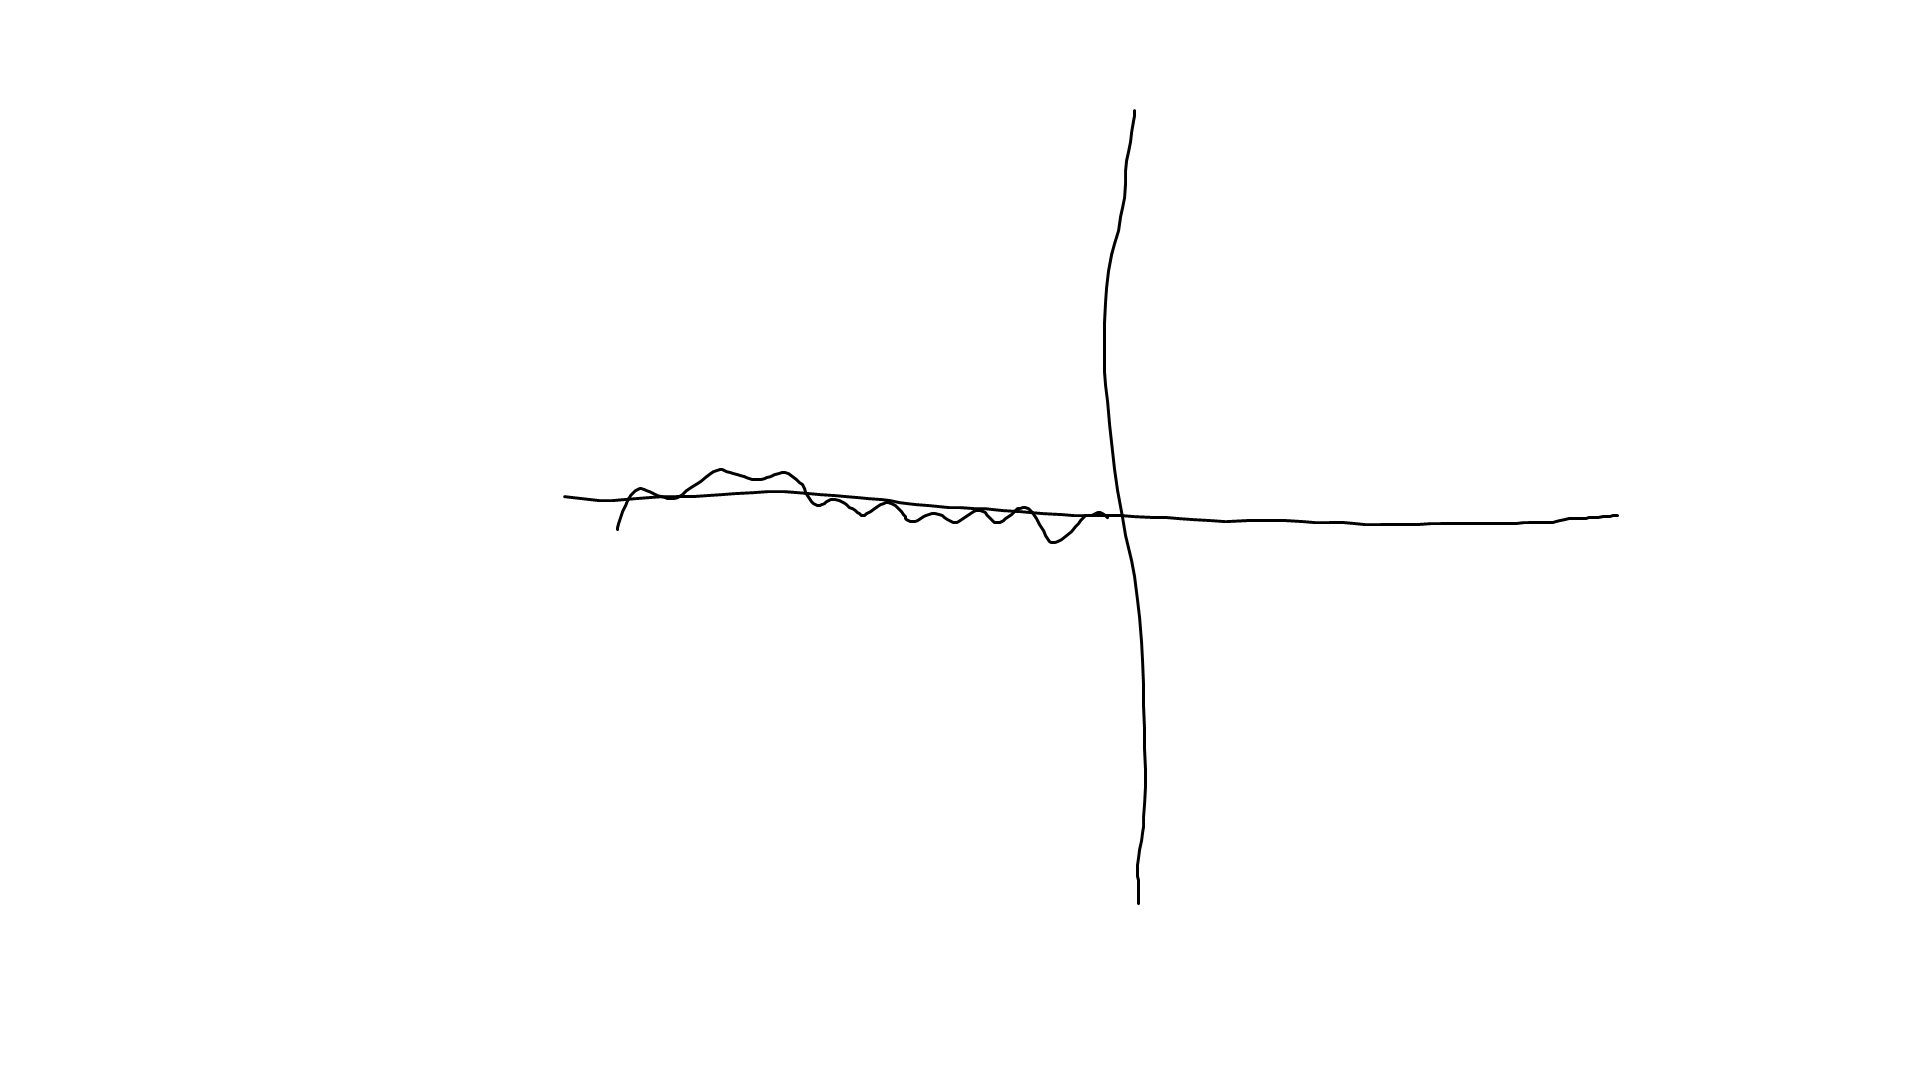
\includegraphics[scale=0.3]{CA_01}

The principal branch of $\log$ is the function $\Log: U \to \C$ given by
\begin{equation*}
\begin{aligned}
\Log(z) = \log|z| + i\arg(z)
\end{aligned}
\end{equation*}
where $\arg(z)$ is the unique argument of $z$ in the range $(-\pi,\pi)$.
\end{defi}

Certainly, $e^{\Log z} = e^{\log z}(\cos\arg(z)+i\sin\arg(z)) = z$.\\
$\Log$ is continuous because $\arg(z):U \to \R$ is continuous.\\
$\C \backslash \{0 \} \to S^1$= unit circle by $z \to \frac{z}{|z|}$ is continuous. This maps $U \to S^1 \backslash \{-1\}$.

$\theta \to e^{i \theta}$ is a homomorphism from $(-\pi,\pi) \to S^1 \backslash \{-1\}$.

\begin{prop} 1.5\\
(i) $\Log z$ is holomorphic in $U$ with derivative $\frac{1}{z}$;\\
(ii) If $|z|<1$, then $\Log(1+z) = \sum_{n=1}^\infty \frac{(-1)^{n-1} z^n}{n}$.
\begin{proof}
(i) Follow from the previous remark.\\
(ii) Note
\begin{equation*}
\begin{aligned}
\frac{d}{dz} \Log(1+z) = \frac{1}{z+1}
\end{aligned}
\end{equation*}
and that the series has radius of convergence $1$. So we can differentiate RHS term by term:
\begin{equation*}
\begin{aligned}
\frac{d}{dz}(\sum_{n=1}^\infty \frac{(-1)^n z^n}{n}) = \sum_{n=1}^\infty (-1)^{n-1}z^{n-1} = \frac{1}{1+z}
\end{aligned}
\end{equation*}
so LHS and RHS have the same derivative, i.e. their difference is a constant. Set $z=0$ we see that they are equal.
\end{proof}

Note: there is no continuous extension of $\Log z$ to $\C \backslash \{0\}$ (consider taking the limit from 2nd quadrant downward and 3rd quadrant upward). Later on we'll see that there is no branch of $\log$ defined on $\C \backslash \{0\}$.

We can also define fractional/complex powers by the formula
\begin{equation*}
\begin{aligned}
z^\alpha = \exp(\alpha \Log z)
\end{aligned}
\end{equation*}
for $z \in U$.

\end{prop}

\subsection{Conformal maps}
Let $f:U \to \C$ be a holomorphic function with $U$ open. Let $w \in U$, if $f'(w) \neq 0$, we say that $f$ is conformal at $w$.

Such an $f$ preserves angles in the following sense: Suppose we have $\gamma_i: [-1,1] \to U$, $C^1$ curves. $\gamma_i(0) = w$< $\gamma'_i(0) \neq 0$. Let $\delta_i(t) = f(\gamma_i(t))$. Then the angles between the two curves at $w$ before and after the map $f$ are the same.

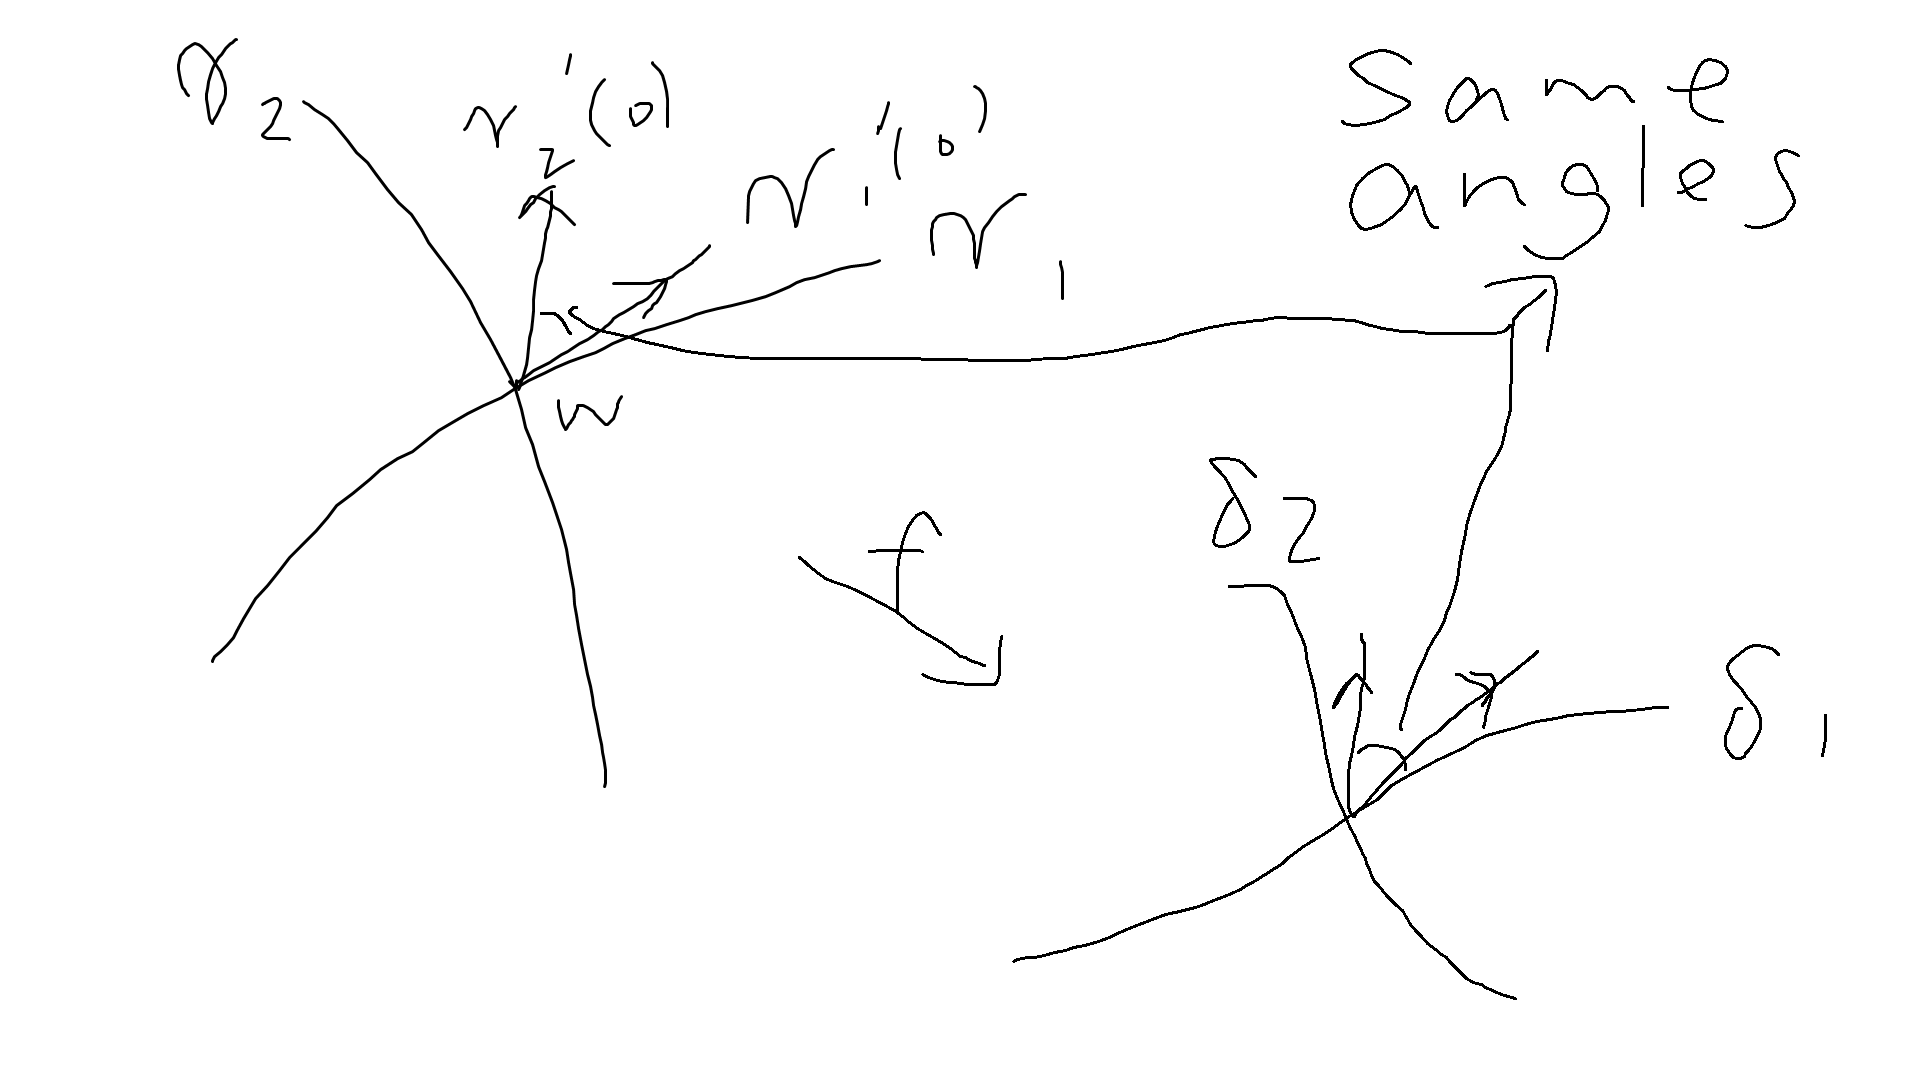
\includegraphics[scale=0.5]{CA_02}

$\delta'_i(0) = f'(w) \gamma'_i(0)$, so
\begin{equation*}
\begin{aligned}
\arg((f \gamma_1)'(0)) - \arg((f\gamma_2)'(0)) = \arg(\gamma'_1(0)) - \arg(\gamma'_2(0))
\end{aligned}
\end{equation*}

\begin{defi}
$f: U \to \C$ is conformal if $f'(w) \neq 0$ $\forall w \in U$.
\end{defi}

\begin{defi}
If $f:D \to \C$ is holomorphic where $D$ is a domain with $f' \neq 0$ everywhere, and $f$ is 1-1 so that $f:D \to f(D)$ is a bijection, then we say that $f$ is a \emph{conformal equivalence} (note: such an $f$ has $f^{-1}$ holomorphic by IVT).

$D$ and $f(D)$ are 'equivalent' from a holomorphic point of view.
\end{defi}

\begin{eg}
(1) Mobius map: endomorphism of $\C \cup \{\infty\}$ by
\begin{equation*}
\begin{aligned}
f(z) = \frac{az + b}{cz + d}, ad-bc \neq 0
\end{aligned}
\end{equation*}
this is a bijection. We see $f'(z) \neq 0$.\\
(2) $z \to z^n$. $\{z \in \C^*, 0 <\arg(z) < \frac{\pi}{n}\} \to \{z \in \C: \Im(z) > 0\}$, for $n \geq 1$. This is conformal on $\C^*$ (for $n \geq 2$, $z \to z^n$ is not conformal at $z=0$).\\
(3) $e^z$ is conformal in all $\C$. If we restrict to the principal branch, then this is a conformal equivalence.
\end{eg}

\begin{thm} (Riemann mapping theorem)\\
Let $D \subset \C$ be any domain bounded by a simple closed curve. Then then there exists a conformal equivalence between $D$ and $D(0,1)$. More generally, such a conformal equivalence exists for any $D$ simply connected, which is not all $\C$.
\end{thm}

\newpage

\section{Complex Integration I}
If $f:[a,b] \to \C$ is continuous, then
\begin{equation*}
\begin{aligned}
\int_a^b f(t) dt = \int_a^b \Re(f(t))dt + i \int_a^b \Im(f(t))dt
\end{aligned}
\end{equation*}

Basic estimate:
\begin{prop} 2.1\\
\begin{equation*}
\begin{aligned}
\left|\int_a^b f(t)dt\right| \leq (b-a) \sup_{t\in[a,b]} |f(t)|
\end{aligned}
\end{equation*}
with equality iff $f$ is constant.
\begin{proof}
Let $\theta = \arg\int a^b f(t) dt$ and set $M = \sup_{t \in [a,b]} |f(t)|$. Then
\begin{equation*}
\begin{aligned}
\left|\int_a^b f(t) dt\right| &= e^{-i\theta} \int_a^b f(t)dt\\
&= \int_a^b e^{-i\theta} f(t)dt\\
&= \int_a^b \Re(e^{-i\theta} f(t)) dt\\
&\leq \int_a^b |f(t)|dt\\
&\leq (b-a)M
\end{aligned}
\end{equation*}
if the equality holds, then all the equality holds along the chain. So $|f(t)|=M$ $\forall t$, and $f(t) = Me^{i\theta}$. So $f$ is constant.
\end{proof}
\end{prop}

Let $\gamma:[a,b] \to \C$ be a $C^1$ curve (i.e. $\gamma^1$ exists and is continuous). We define the length of $\gamma$ to be
\begin{equation*}
\begin{aligned}
l = \int_a^b |\gamma'(t)|dt
\end{aligned}
\end{equation*}
$\gamma$ is \emph{simple} if $\gamma(t_1) \neq \gamma(t_2)$ unless $t_1 = t_2$ or $\{t_1,t_2\} = \{a,b\}$.

\begin{defi}
$f:U \to \C$ is continuous, $\gamma:[a,b] \to U$ is a $C^1$ curve. Then the integral of $f$ along $\gamma$ is
\begin{equation*}
\begin{aligned}
\int_\gamma f(z) dz = \int_a^b f(\gamma(t)) \gamma'(t) dt
\end{aligned}
\end{equation*}
\end{defi}

Basic properties:\\
(1) Linearity:
\begin{equation*}
\begin{aligned}
\int_\gamma (c_1 f_1(z) + c_2 f_2(z)) dz = c_1 \int_\gamma f_1(z)dz + c_2\int_\gamma f_2(z) dz
\end{aligned}
\end{equation*}
(2) if $a < a' < b$, then
\begin{equation*}
\begin{aligned}
\int_\gamma f(z) dz = \int_{\gamma|_{[a,a']}} f(z) dz + \int_{\gamma|_{[a',b]}} f(z) dz
\end{aligned}
\end{equation*}
(3) Inverse path: if $(-\gamma):[-b,-a] \to U$ is the curve
\begin{equation*}
\begin{aligned}
(-\gamma)(t) = \gamma(-t)
\end{aligned}
\end{equation*}
then
\begin{equation*}
\begin{aligned}
\int_{-\gamma} f(z) dz = -\int_\gamma f(z) dz
\end{aligned}
\end{equation*}
(4) Independent of re-parameterization: if $\phi:[a',b'] \to [a,b]$ is $C^1$ and $\phi(a')=a$, $\phi(b') = b$, then if $\delta = \gamma \circ \phi: [a',b'] \to U$, then we have
\begin{equation*}
\begin{aligned}
\int_\gamma f(z) dz = \int_\delta f(z) dz
\end{aligned}
\end{equation*}
This is because $\delta' = \gamma' \phi'$,
\begin{equation*}
\begin{aligned}
\int_\delta f(z) dz = \int_{a'}^{b'} f(\gamma(\phi(t)))\gamma'(\phi(t))\phi'(t) dt
\end{aligned}
\end{equation*}
Substitution $s=\phi(t)$ gives $\int_\gamma f(z) dz$.

Let $\gamma: [a,b] \to \C$ be a continuous curve. Suppose we have $a=a_0<a_1<...<a_{n-1}<a_n = b$ s.t. $\gamma_i := \gamma|_{[a_{i-1},a_i]}$ is $C^1$ for $1\leq i \leq n$. Then we say that $\gamma$ is \emph{piecewise $C^1$} and define
\begin{equation*}
\begin{aligned}
\int_\gamma f(z) dz = \sum_{i=1}^n \int_{\gamma_i}f(z) dz
\end{aligned}
\end{equation*}

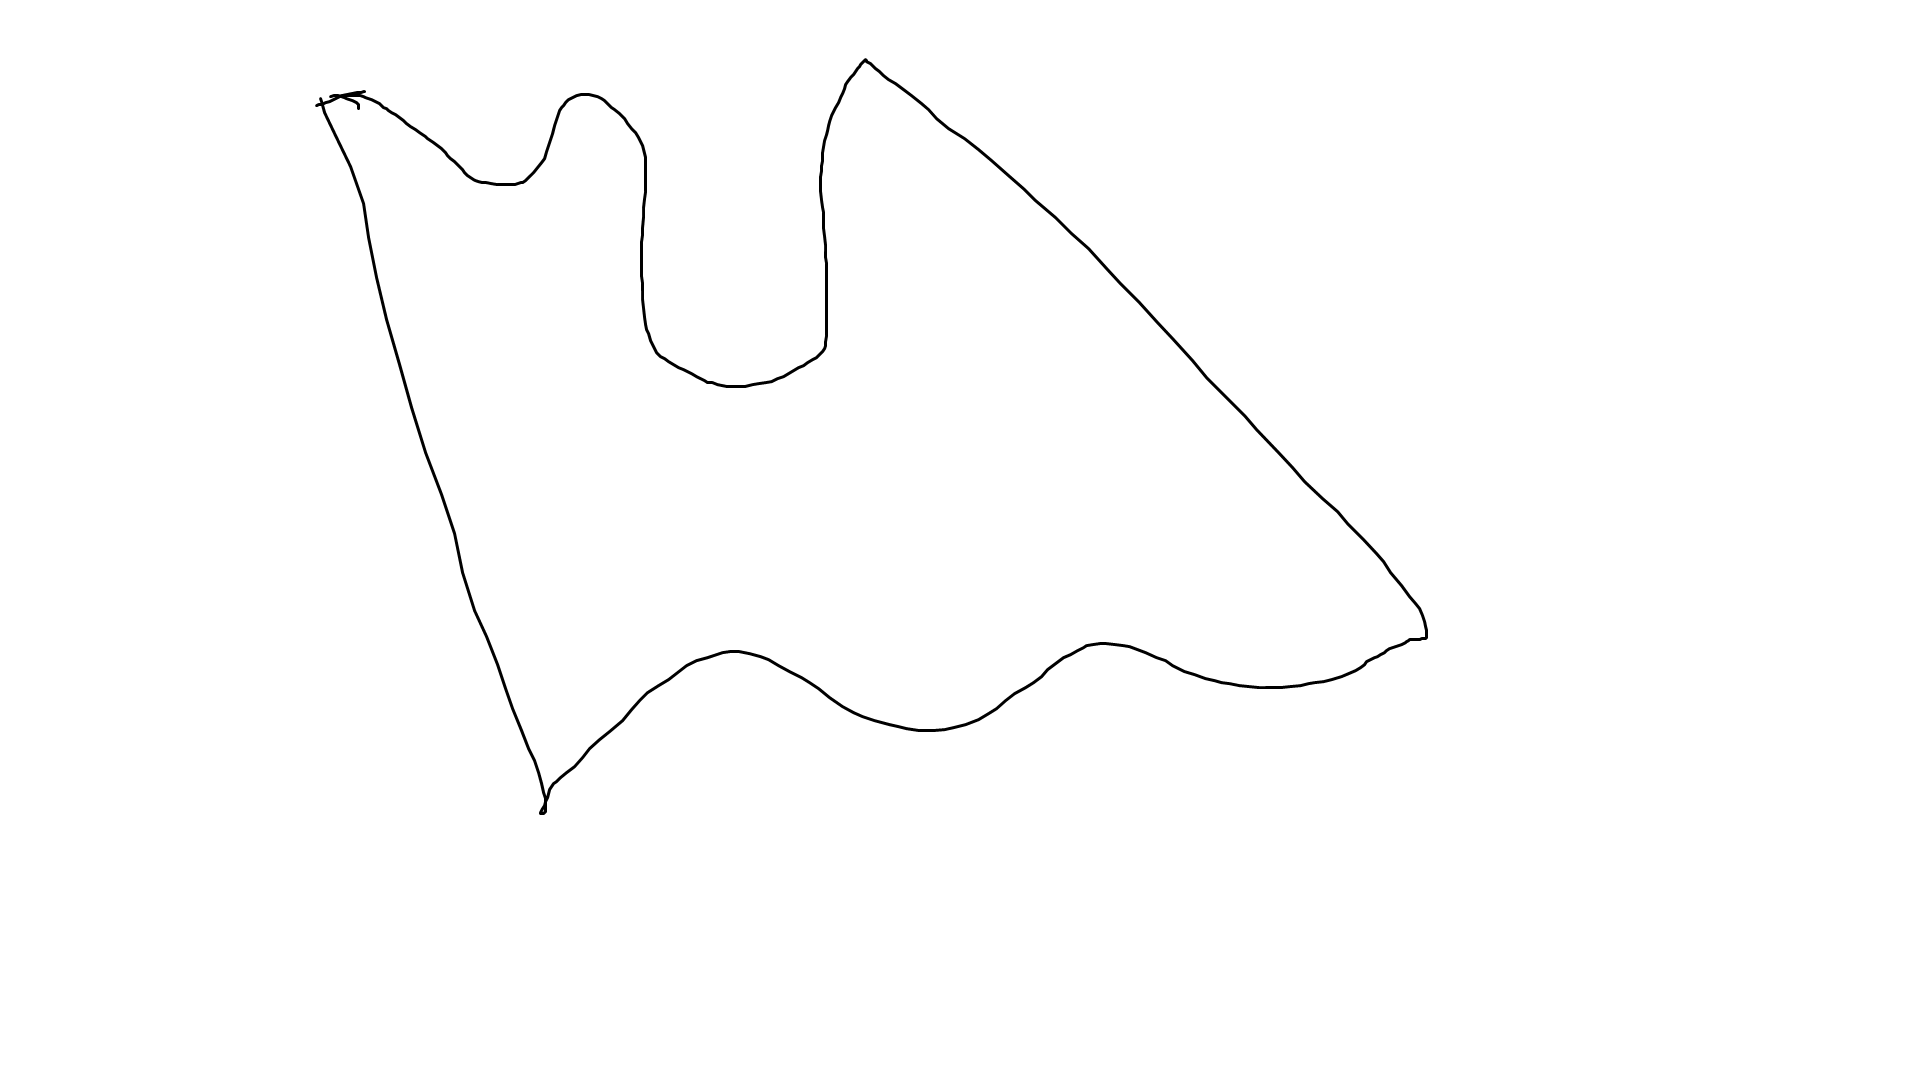
\includegraphics[scale=0.3]{CA_03}

\begin{eg}
(1) $f(z) = z^n$, $U = \C^*$, $n \in \Z$. Consider $\gamma:[0,2\pi] \to U$ by $t \to e^{it}$, then $\gamma' =ie^{it}$. 

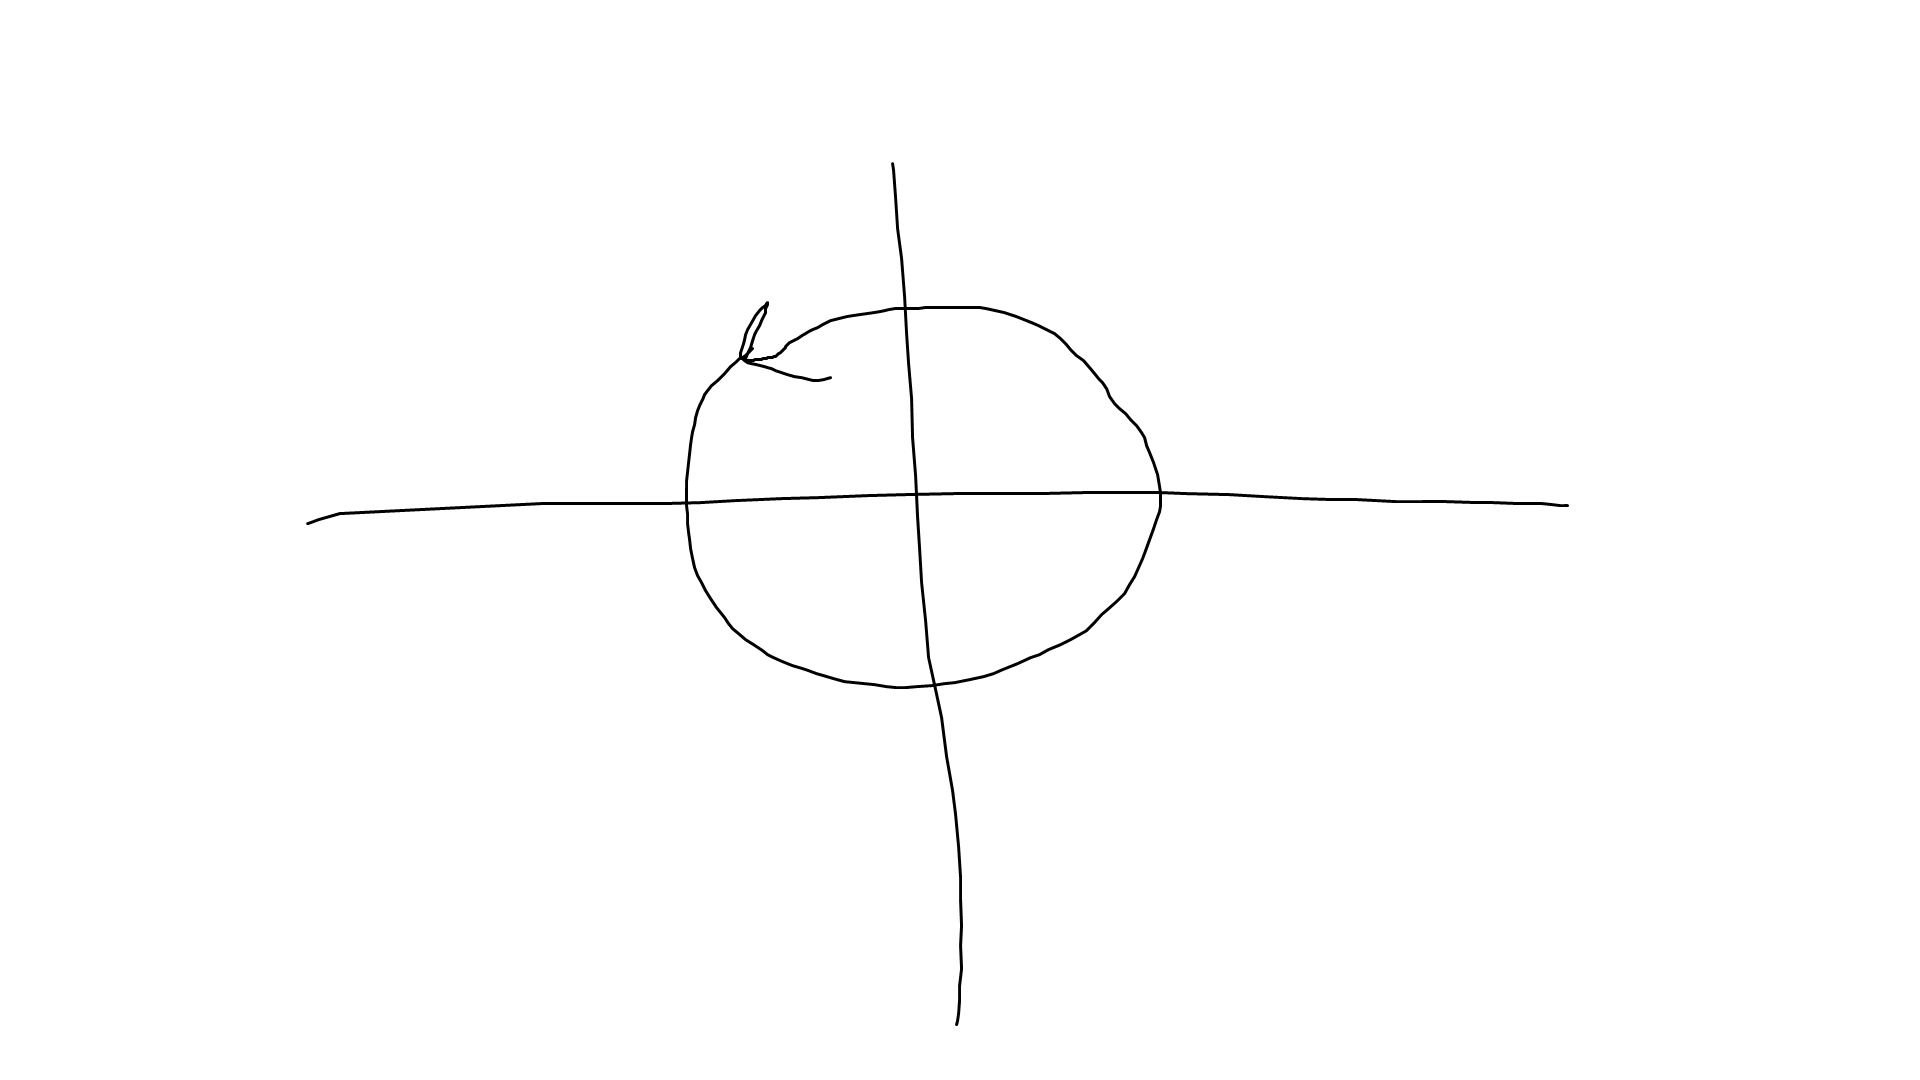
\includegraphics[scale=0.3]{CA_04}

We have
\begin{equation*}
\begin{aligned}
\int_\gamma f(z) dz &= \int_0^{2\pi} e^{int}ie^{it} dt\\
&= i\int_0^{2\pi} e^{i(n+1)t}dt\\
&= \left\{ \begin{array}{ll}
2\pi i & n=-1\\
0 & n\neq -1
\end{array}\right.
\end{aligned}
\end{equation*}
(2) $f(z)=z^2$, $\gamma_1: [-R,R] \to \C$, $\gamma_1(t) = t$; $\gamma_2: [0,1] \to \C$, $\gamma_2(t) = Re^{i\pi t}$. 

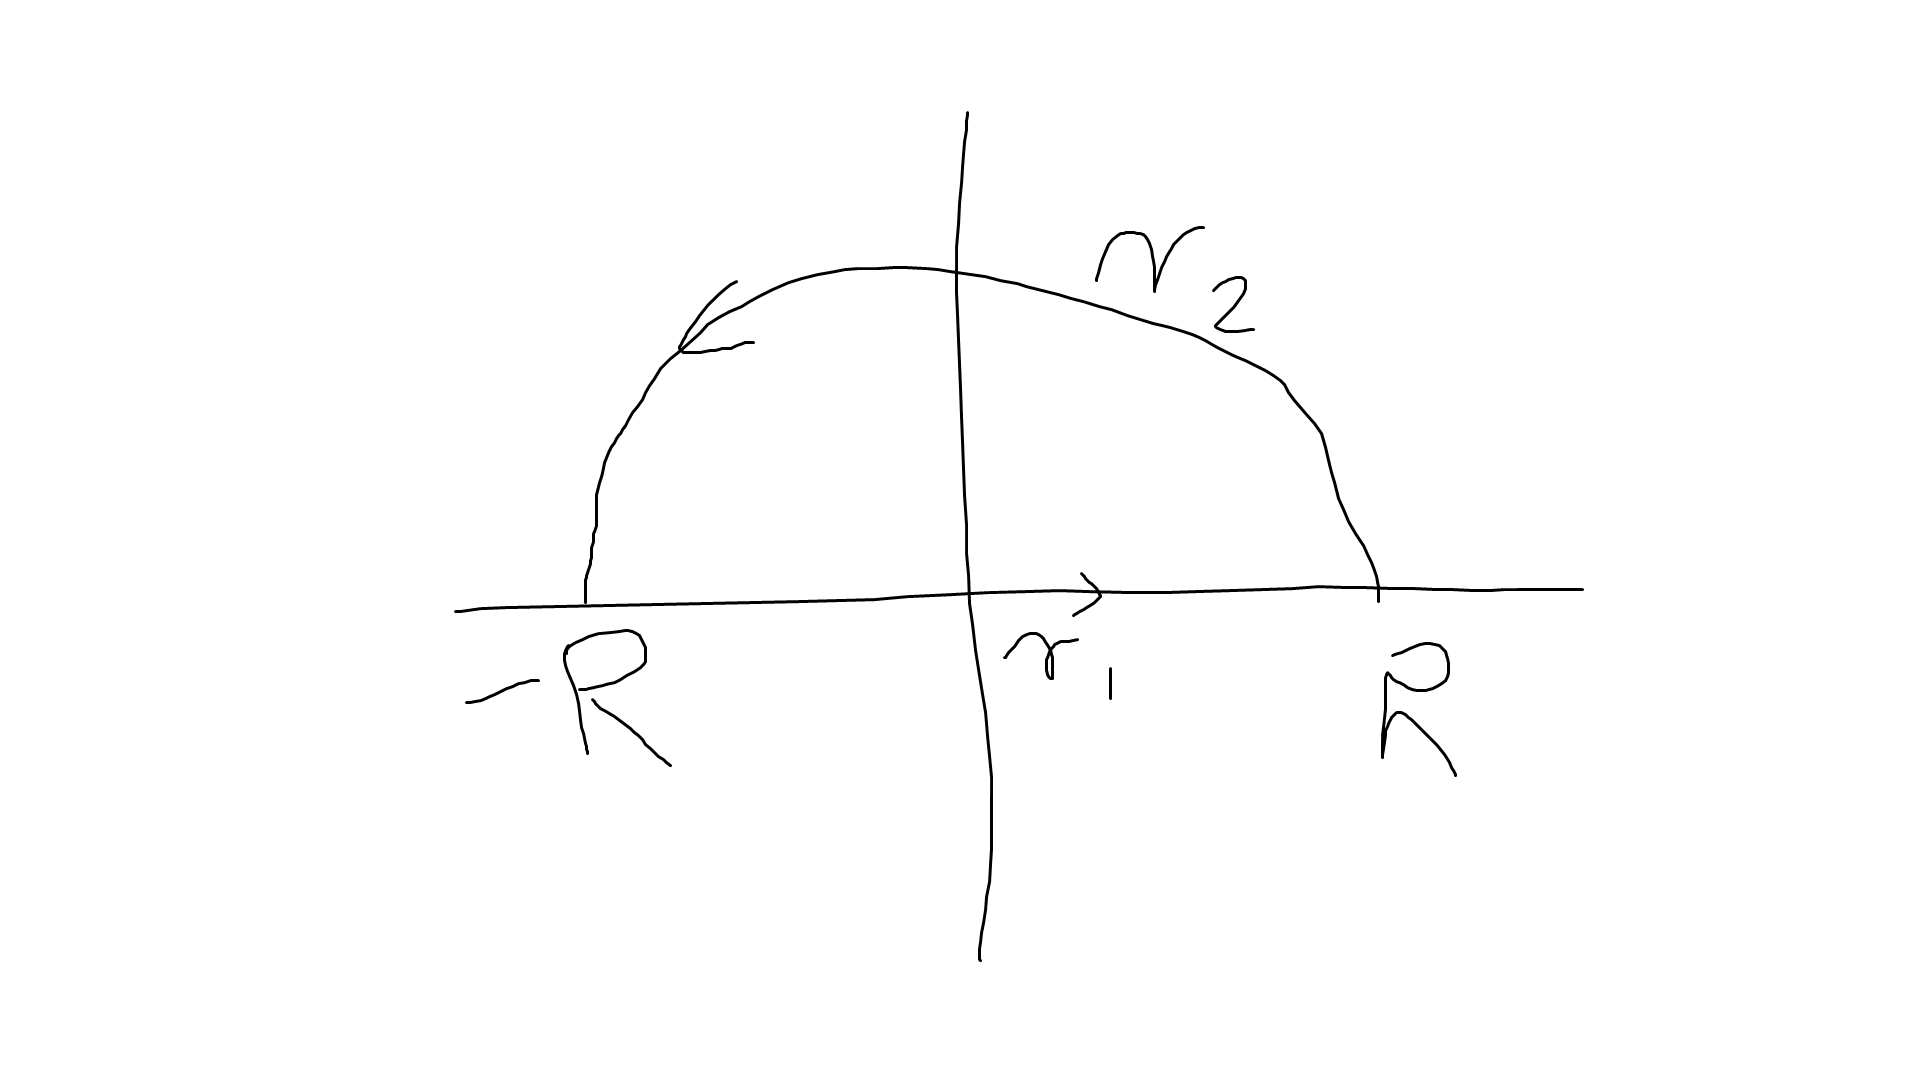
\includegraphics[scale=0.3]{CA_05}

We have
\begin{equation*}
\begin{aligned}
\int_\gamma f(z) dz &= \int_{\gamma_1} f(z) dz + \int_{\gamma_2} f(z) dz\\
&= \int_{-R}^R t^2 dt + \int_0^1 R^2 e^{2\pi it} i\pi R e^{i\pi t} dt\\
&= \frac{2R^3}{3} + \left(-\frac{2R^3}{3}\right)\\
&= 0
\end{aligned}
\end{equation*}
\end{eg}

\begin{prop} 2.2\\
For any continuous $f:U \to \C$ ($U$ open) and any curve $\gamma: [a,b] \to U$, we have
\begin{equation*}
\begin{aligned}
\left| \int_\gamma f(z) dz\right| \leq length(\gamma) \sup_\gamma |f| (= \sup_{t\in [a,b]} |f(\gamma(t))|)
\end{aligned}
\end{equation*}
\begin{proof}
WLOG assume $\gamma$ is $C^1$ and let $M = \sup_\gamma |f|$. Then
\begin{equation*}
\begin{aligned}
\left|\int_\gamma f(z) dz\right| &= \left|\int_a^b f(\gamma(t))\gamma'(t) dt\right|\\
&\leq \int_a^b |f(\gamma(t))||\gamma'(t)| dt\\
&\leq M\int_a^b |\gamma'(t)| dt\\
&= M length(\gamma).
\end{aligned}
\end{equation*}
\end{proof}
\end{prop}

\begin{thm} 2.3 \\(Fundamental theorem of Calculus) \\
Suppose $f:U \to \C$ is continuous and $\exists$ $F(z)$ s.t. $F'(z) = f(z)$ $\forall z \in U$. Then for any curve $\gamma:[a,b] \to U$,
\begin{equation*}
\begin{aligned}
\int_\gamma f(z) dz = F(\gamma(b)) - F(\gamma(a)).
\end{aligned}
\end{equation*}
Such $F$ is called an \emph{anti-derivative} of $f$ on $U$.
\end{thm}

\begin{proof}
\begin{equation*}
\begin{aligned}
\int_\gamma f(z) dz &= \int_a^b f(\gamma(t)) \gamma'(t) dt\\
&=F(\gamma(b)) - F(\gamma(a)).
\end{aligned}
\end{equation*}
\end{proof}

\begin{coro} 2.4\\
If $\gamma$ is \emph{closed} ($\gamma(b) = \gamma(a)$) and $f$ is continuous with anti-derivative $F$ on $U \supset \gamma([a,b])$, then
\begin{equation*}
\begin{aligned}
\int_\gamma f(z) dz = 0.
\end{aligned}
\end{equation*}
\end{coro}

Look at $f(z) = z^n$ for $n \in \Z$. Then
\begin{equation*}
\begin{aligned}
\int_\gamma z^n dz = \left\{ \begin{array}{ll}
0 & n \neq -1\\
2\pi i & n = -1
\end{array}\right.
\end{aligned}
\end{equation*}
If $n \neq -1$, $z^n$ = $\frac{d}{dz}\left(\frac{z^{n+1}}{n+1}\right)$, so the result $0$ is expected by the above corollary. However if $n=-1$, then $\frac{1}{z}$ does not have an anti-derivative on $\C^*$ (no branch of $\log$ on $\C^*$).

\begin{prop} 2.5\\
Let $U \subset \C$ be a domain. If $f: U \to \C$ is continuous and
\begin{equation*}
\begin{aligned}
\int_\gamma f(z) dz =0 
\end{aligned}
\end{equation*}
for all closed paths $\gamma$ in $U$, then $f$ has an anti-derivative $F$ on $U$.
\begin{proof}
Pick $a_0 \in U$. Since $U$ is a domain, for each $w \in U$ we can pick a path $\gamma_w:[0,1] \to U$ s.t. $\gamma_w(0) = a_0$, $\gamma_w(1) = w$.

Let
\begin{equation*}
\begin{aligned}
F(w) = \int_{\gamma_w} f(z) dz
\end{aligned}
\end{equation*}
Note $F$ is independent of the choice of $\gamma_w$ by hypothesis.

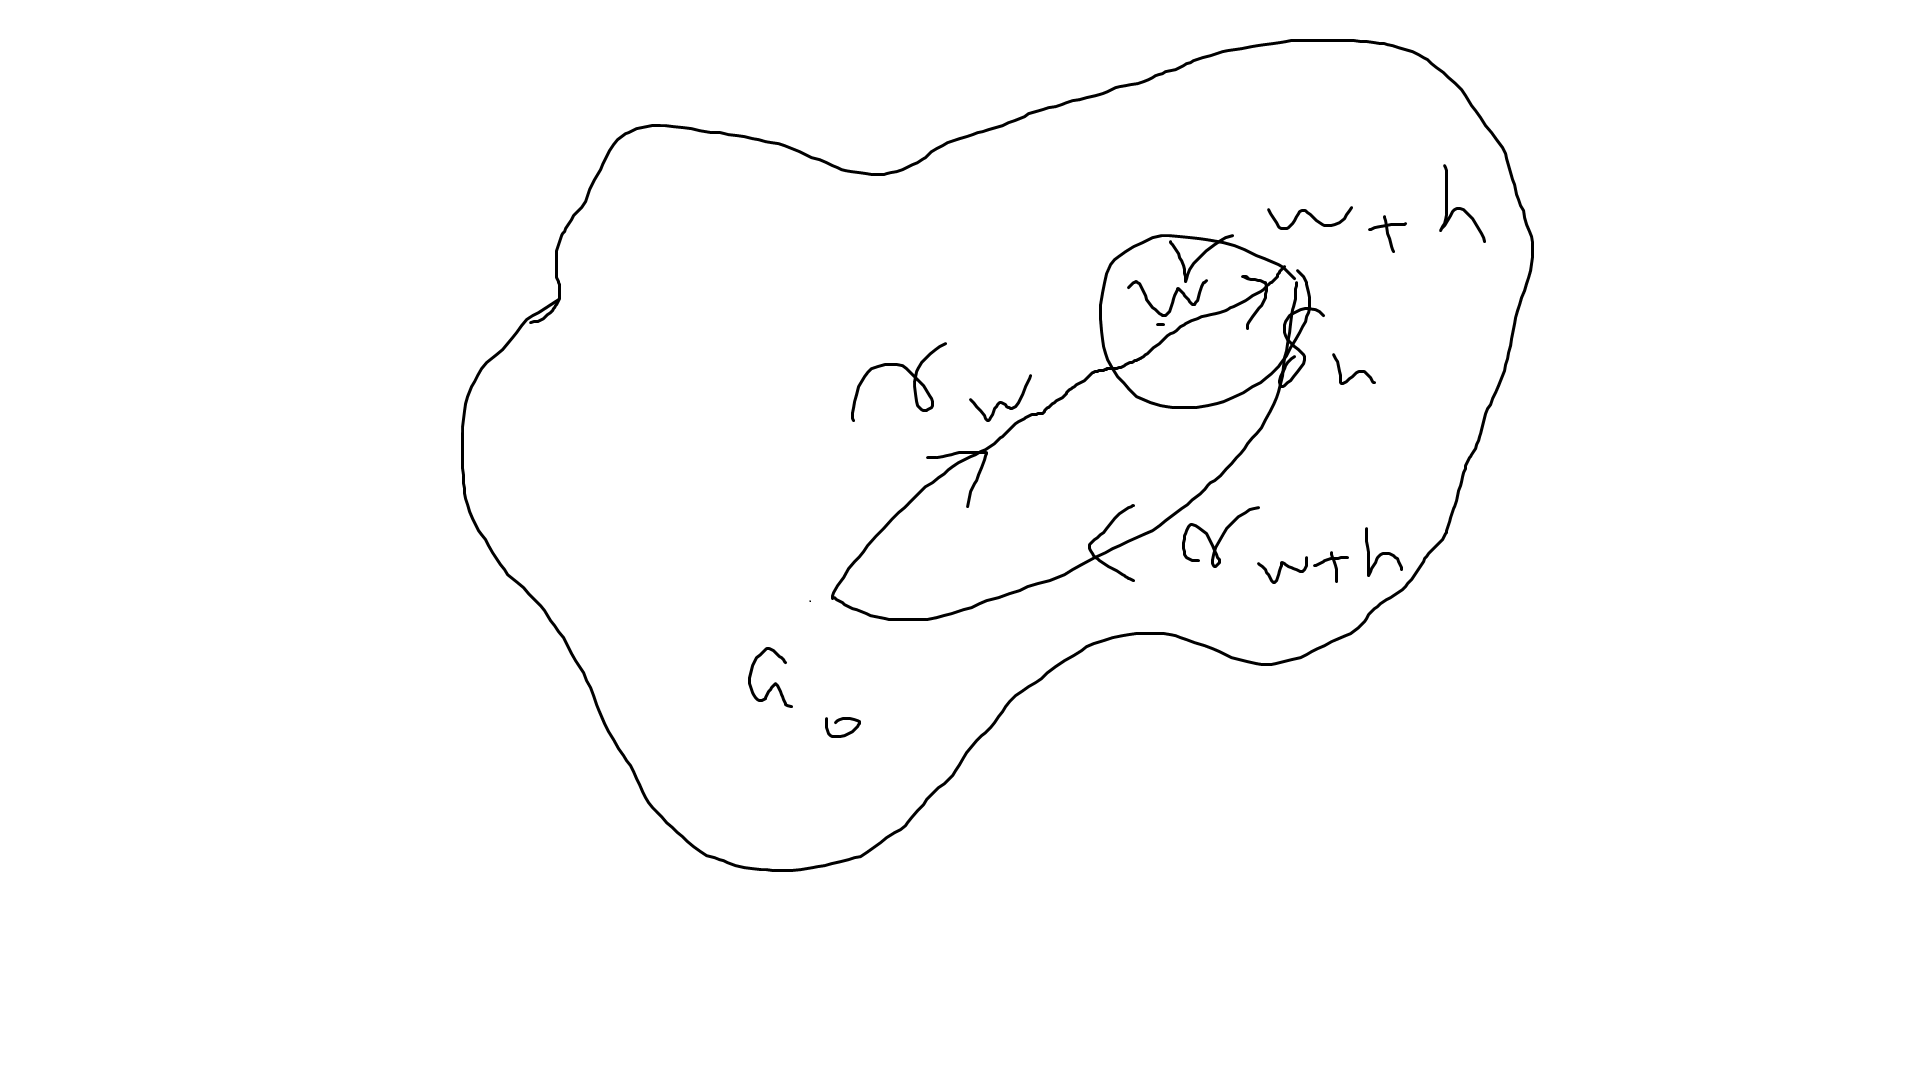
\includegraphics[scale=0.4]{CA_06}

We claim $F$ is holomorphic and $F' = f$.

Since $U$ is open, $\exists r>0$ s.t. $D(w,r) \subset U$. Let $h$ be s.t. $|h|<r$ and let $\delta_h$ be the radial path from $w$ to $w+h$. 

Let $\gamma = \gamma_w * \delta_h * (-\gamma_{w+h})$ be concatenation of paths. $\gamma$ is closed. So
\begin{equation*}
\begin{aligned}
\int_\gamma f(z) dz = 0
\end{aligned}
\end{equation*}
i.e.
\begin{equation*}
\begin{aligned}
F(w+h) &= \int_{\gamma_w * \delta_h} f(z) dz\\
&=F(w) + \int_{\delta_h} f(z) dz\\
&= F(w) + hf(w) + \int_{\delta_h} (f(z)-f(w)) dz.
\end{aligned}
\end{equation*}
So
\begin{equation*}
\begin{aligned}
\left|\frac{F(w+h)-F(w)}{h} - f(w)\right| &= \frac{1}{|h|} \left|\int_{\delta_h} (f(z)-f(w)) dz\right|\\
& \leq \frac{length(\delta_h)}{|h|} \sup_{z \in \delta_h} |f(z)-f(w)|\\
&\to 0
\end{aligned}
\end{equation*}
as $h \to 0$ by continuity of $f$.
\end{proof}
\end{prop}

\begin{defi}
A domain $U$ is \emph{star-shaped} (star-domain) if $\exists p \in U$ s.t. $\forall a \in U$, the straight segment $[a,p] \subset U$.

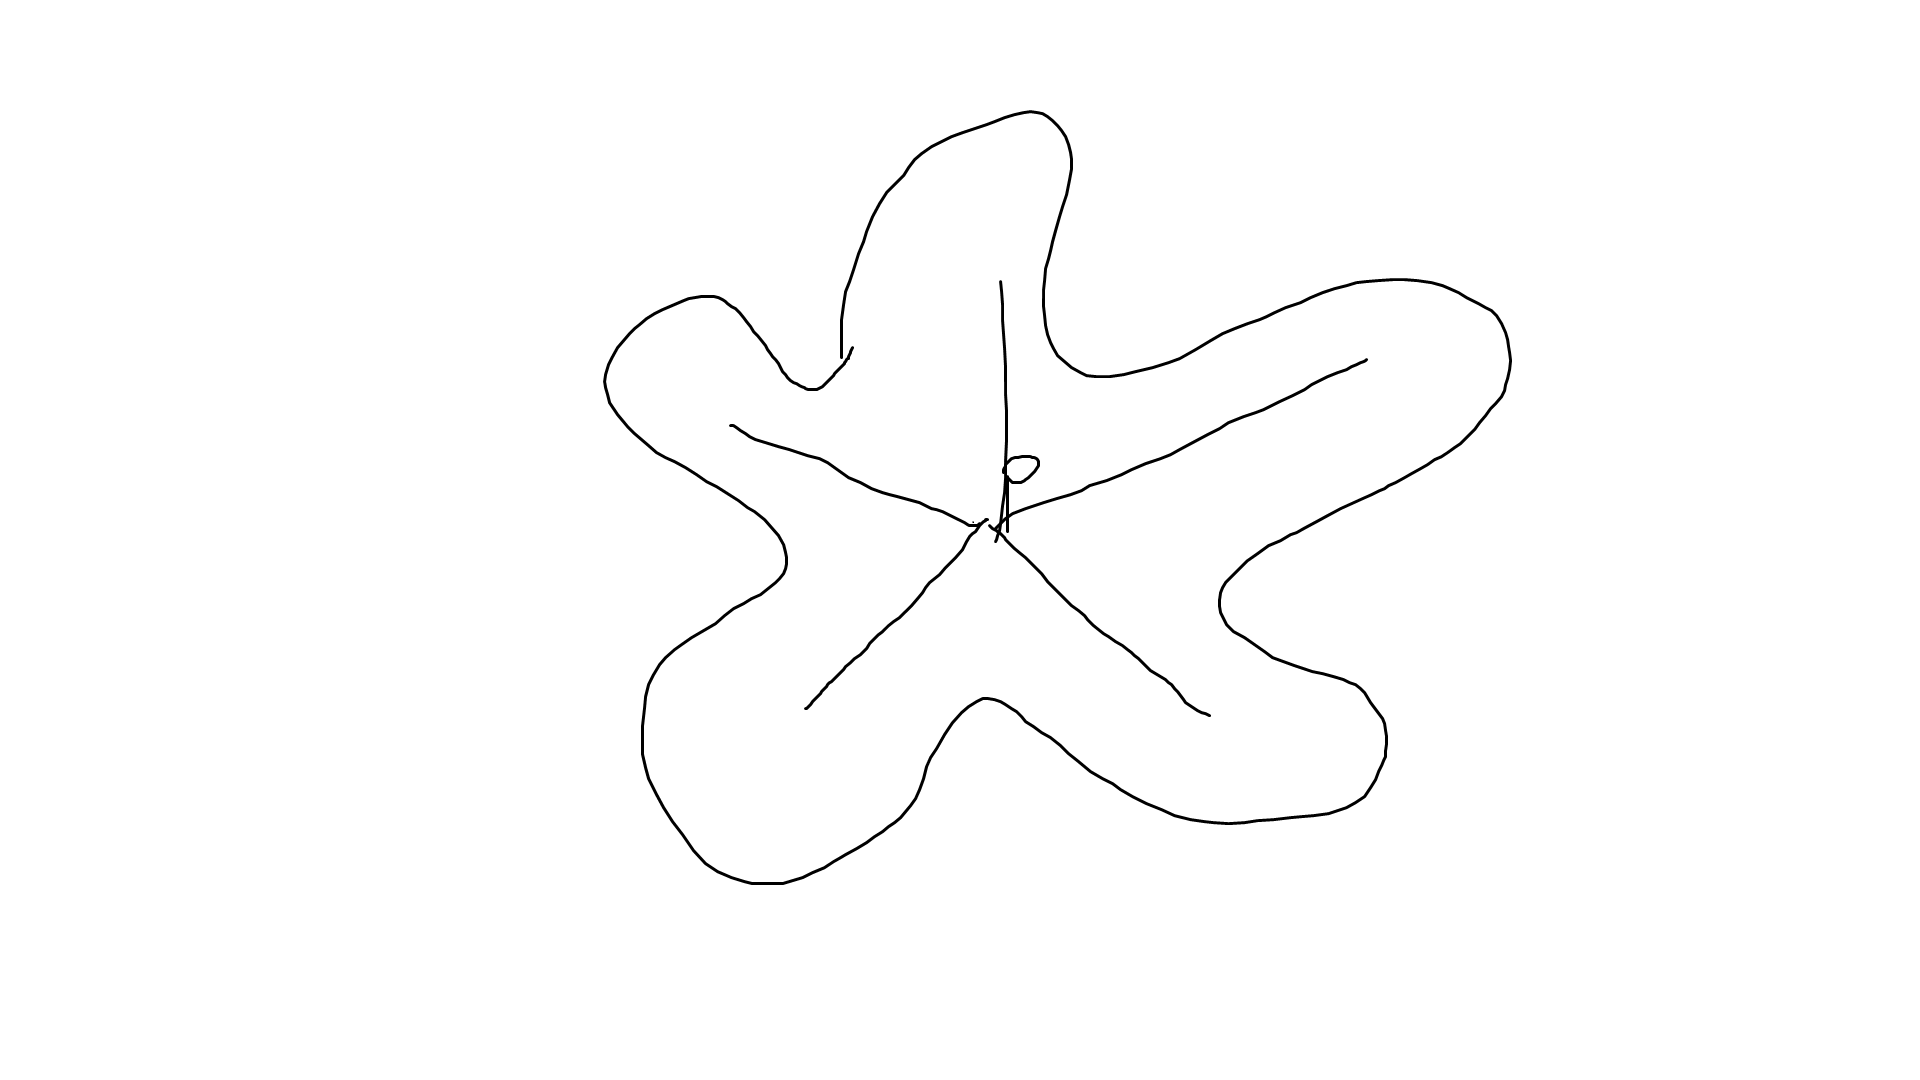
\includegraphics[scale=0.4]{CA_07}
\end{defi}

\begin{eg}
A disc is convex, so is star-shaped, so is a domain.
\end{eg}

\begin{coro} 2.6\\
If $U$ is star-shaped, $f: U \to \C$ is continuous and
\begin{equation*}
\begin{aligned}
\int_\gamma f(z) dz = 0
\end{aligned}
\end{equation*}
for all \emph{triangles} $\gamma \subset U$, then $f$ has an anti-derivative on $U$.
\begin{proof}
If $U$ is star-shaped, then about $p$, let $\gamma_\omega = [p,\omega]$ $\forall \omega \in U$. The previous proof works since $\gamma_\omega * \delta_h * (-\gamma_{\omega+h})$ is a triangle.
\end{proof}
\end{coro}

\begin{thm} 2.7 (Cauchy's Theorem for Triangles)\\
Let $U$ be a domain. Let $T \subset U$ be a triangle. If $f:U \to \C$ is holomorphic, then
\begin{equation*}
\begin{aligned}
\int_{\partial T} f(z) dz = 0
\end{aligned}
\end{equation*}
\begin{proof}
Let
\begin{equation*}
\begin{aligned}
\eta = \left| \int_{\partial T} f(z) dz\right|,
\end{aligned}
\end{equation*}
$l = length(\partial T)$. Let $T^0 = T$ and subdivide into 4 equal triangles $T = T_1 \cup ... \cup T_4$. Then
\begin{equation*}
\begin{aligned}
\end{aligned}
\end{equation*}
Then
\begin{equation*}
\begin{aligned}
\int_{\partial T} f(z) dz = \sum_{i=1}^4 \int_{\partial T_i} f(z) dz
\end{aligned}
\end{equation*}
as internal lines cancel in pairs.

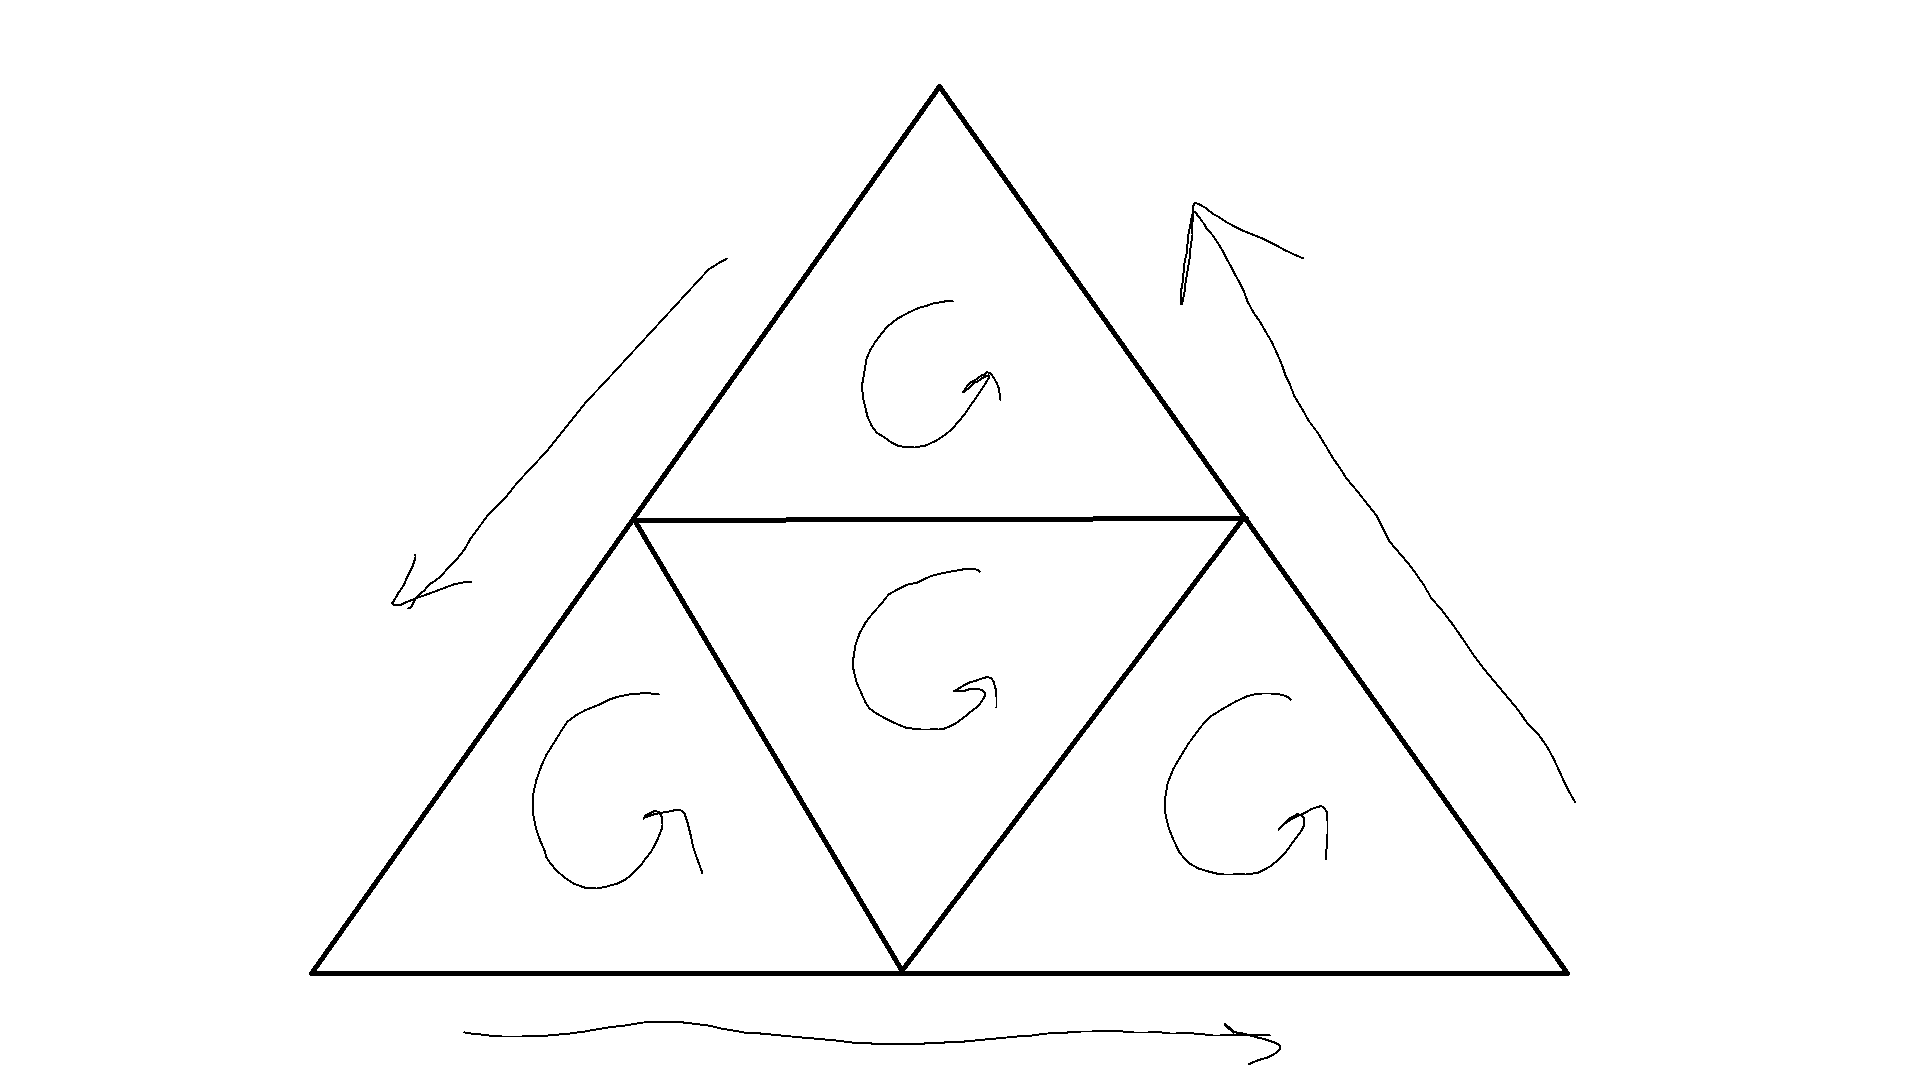
\includegraphics[scale=0.4]{CA_08}

So, $\exists i$, $1 \leq i \leq 4$, s.t.
\begin{equation*}
\begin{aligned}
\left|\int_{\partial T_i} f(z) dz\right| \geq \frac{\eta}{4}.
\end{aligned}
\end{equation*}
Let $T^1 = T_i$ for this $i$, and repeat. We produce a sequence $T^0,T^1,...$ s.t.
\begin{equation*}
\begin{aligned}
\left|\int_{\partial T^i} f(z) dz\right| \geq \frac{\eta}{4^i},
\end{aligned}
\end{equation*}
and
\begin{equation*}
\begin{aligned}
length(\partial T^i) =\frac{l}{2^i}.
\end{aligned}
\end{equation*}

We observe that 
\begin{equation*}
\begin{aligned}
\bigcap_{i=0}^\infty T^i \neq \phi
\end{aligned}
\end{equation*}
since $T^0$ is compact. So there exists
\begin{equation*}
\begin{aligned}
z_0 \in \bigcap_{i=0}^\infty T^i
\end{aligned}
\end{equation*}

Since $f$ is differentiable at $z_0$, given $\varepsilon>0$, $\exists \delta>0$ s.t.
\begin{equation*}
\begin{aligned}
|w-z_0|<\delta \implies |f(w)-f(z_0) - (w-z_0)f'(z_0)| < \varepsilon|w-z_0|
\end{aligned}
\end{equation*}

Pick $n$ s.t. $T^n \subset D(z_0,\delta)$. Then
\begin{equation*}
\begin{aligned}
\frac{\eta}{4^n} &\leq \left|\int_{\partial T^n} f(z) dz\right|\\
&= \left|\int_{\partial T^n} (f(z)-f(z_0))-(z-z_0)f'(z_0)dz\right|
\end{aligned}
\end{equation*}
This is because
\begin{equation*}
\begin{aligned}
\int_{\partial T^n} dz = \int_{\partial T^n} zdz = 0
\end{aligned}
\end{equation*}
(1 and $z$ have primitive, $z$, $\frac{z^2}{2}$). Continuing, using estimate from last lecture,
\begin{equation*}
\begin{aligned}
RHS &\leq length(\partial T^n) \varepsilon \sup_{z \in \partial T^n} |z-z_0|\\
&\leq [length(\partial T^n)]^2 \varepsilon \\
&= \frac{l^2}{4}\varepsilon
\end{aligned}
\end{equation*}
So
\begin{equation*}
\begin{aligned}
\eta \leq \varepsilon l^2
\end{aligned}
\end{equation*}
But $\varepsilon$ is arbitrary. So $\eta = 0$.
\end{proof}
\end{thm}

\begin{coro} 2.8 (Convex Cauchy)\\
Let $f$ be a holomorphic function on a star-shaped domain $U$. Then
\begin{equation*}
\begin{aligned}
\int_\gamma f(z) dz = 0
\end{aligned}
\end{equation*}
for all curves $\gamma$ on $U$.
\begin{proof}
by the previous theorem,
\begin{equation*}
\begin{aligned}
\int_{\partial T} f(z) dz = 0
\end{aligned}
\end{equation*}
for all triangles. So by 2.6, $f$ has an anti-derivative $F$ on $U$. Then by Fundamental Theorem of Calculus we get the desired result.
\end{proof}
\end{coro}

\textbf{Addendum.} Suppose $U$ is star-shaped and $S \subset U$ is a finite set. Let $f: U \to \C$ be continuous and holomorphic. on $U\backslash S$. Then the conclusion of Cauchy's theorem still holds, i.e. 
\begin{equation*}
\begin{aligned}
\int_\gamma f(z) dz = 0
\end{aligned}
\end{equation*}
for all curves $\gamma$.
\begin{proof}
Suffices to prove that 
\begin{equation*}
\begin{aligned}
\int_{\partial T} f(z) dz = 0
\end{aligned}
\end{equation*}
$\forall T$. Let $M=\sup_T |f|$. Subdivide $T$ into $r^n$ equal subtriangles, as in the proof of Theorem 2.7.\\
Let $T' \subset T$ be a subtriangle. If $T' \cap S = \phi$, then the proof of 2.7 gives the result. Otherwise, for any $T'$,
\begin{equation*}
\begin{aligned}
\left|\int_{\partial T'} f(z) dz\right| \leq l 2^{-n} M
\end{aligned}
\end{equation*}
Each element of $S$ belongs to at most 6 subtriangle, so this gives
\begin{equation*}
\begin{aligned}
\left|\int_{\partial T} f(z) dz\right| \leq \sum_{T'} \left|\int_{\partial T'} f(z) dz\right| \frac{\leq 6 (\#S) lM}{2^n}
\end{aligned}
\end{equation*}
let $n \to \infty$ we get the desired result.
\end{proof}

\begin{thm} 2.9 (Cauchy's integral formula for a disc)\\
Let $D = D(a,r)$ be a disc, and suppose $f:D \to \C$ is holomorphic. For every $w \in D$ and $\rho$ with $|w-a|<\rho<r$, we have
\begin{equation*}
\begin{aligned}
f(w) = \frac{1}{2\pi i}\int_{|z-a|=\rho} \frac{f(z)}{z-w} dz
\end{aligned}
\end{equation*}

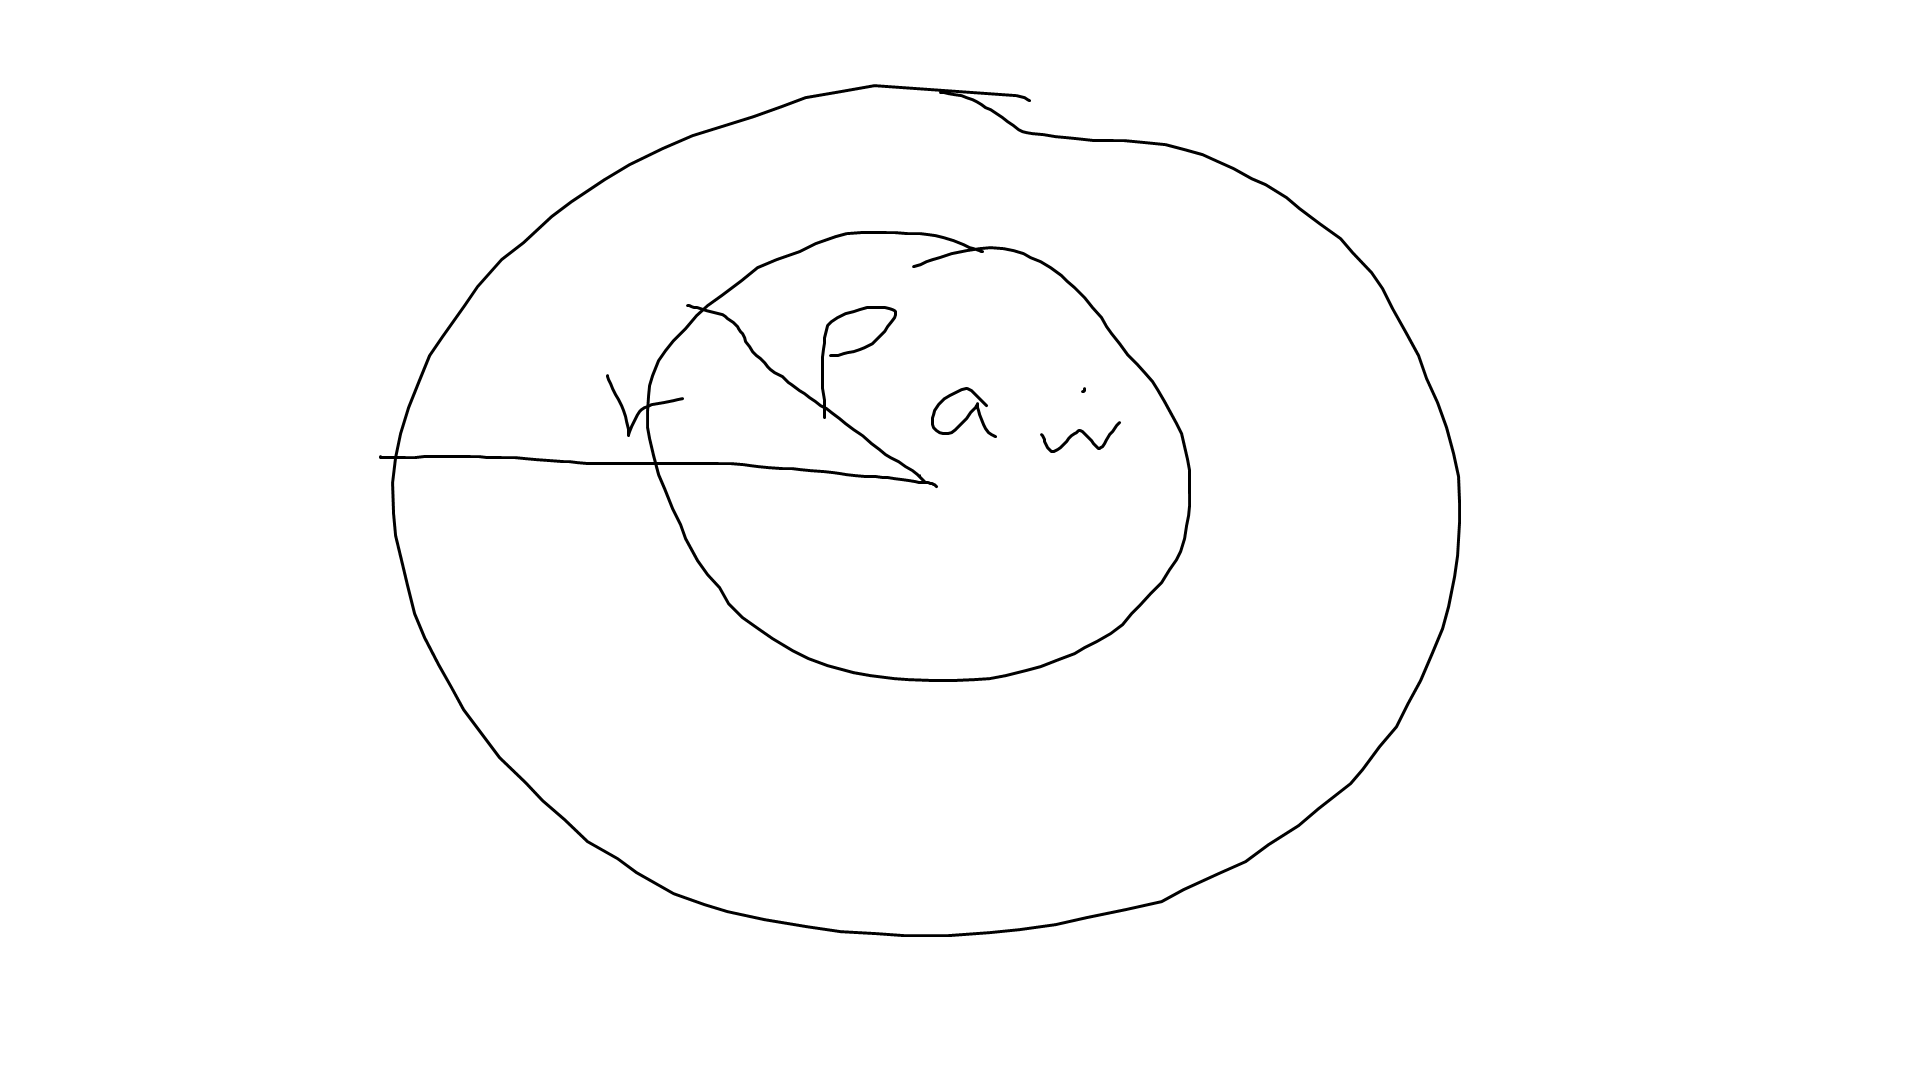
\includegraphics[scale=0.4]{CA_09}
\begin{proof}
Consider the function
\begin{equation*}
\begin{aligned}
g(z) = \left\{ \begin{array}{ll}
\frac{f(z)-f(w)}{z-w} & z\neq w\\
f'(w) & z=w
\end{array}\right.
\end{aligned}
\end{equation*}
Apply the Addendum to $g$ to derive
\begin{equation*}
\begin{aligned}
\int_{|z-a|=\rho} g(z) dz = 0
\end{aligned}
\end{equation*}
So
\begin{equation*}\tag{*}
\begin{aligned}
\int_{|z-a|=\rho} \frac{f(z)}{z-w}dz = \int_{|z-a|=\rho} \frac{f(w)}{z-w}dz
\end{aligned}
\end{equation*}
To compute (*), note the following
\begin{equation*}
\begin{aligned}
\frac{1}{z-w} &= \frac{1}{(z-a)\left(1-\frac{w-a}{z-a}\right)}\\
&= \sum_{n=0}^\infty \frac{(w-a)^n}{(z-a)^{n+1}}
\end{aligned}
\end{equation*}
since $\left|\frac{w-a}{z-a}\right|<1$. Now recall
\begin{equation*}
\begin{aligned}
\int_\gamma z^n dz = \left\{\begin{array}{ll}
2\pi i & n = -1\\
0 & n \neq -1
\end{array}\right.
\end{aligned}
\end{equation*}
So
\begin{equation*}
\begin{aligned}
\int_{|z-a|=\rho} \frac{f(w)}{z-w} dz = \sum_{n=0}^\infty \int_{|z-a|=\rho} f(w) \frac{(w-a)^n}{(z-a)^{n+1}}dz = 2\pi i f(w).
\end{aligned}
\end{equation*}
where the second equality is just the calculation as in the example of $z^n$ ($n \in \Z$ from previous lecture. The first needs justification:
\begin{lemma}
If $f_n: U \to \C$ and $f:U \to \C$ continuous and $\gamma:[a,b] \to U$ a curve s.t. $f_n \to f$ uniformly on $im(\gamma)$, then
\begin{equation*}
\begin{aligned}
\int_\gamma f_n(z) dz \to \int_\gamma f(z) dz
\end{aligned}
\end{equation*}
\end{lemma}
Hence the proof of Cauchy's formula is completed if we can prove this lemma.
\end{proof}
\end{thm}

\textbf{Proof of lemma}: Let $M_n = \sup_\gamma |f_n-f|$. Uniform convergence just says that $M_n \to 0$ as $n \to \infty$. Then from
\begin{equation*}
\begin{aligned}
\left|\int_\gamma (f_n(z) - f(z)) dz \right| & \leq M_n length(\gamma) \to 0.
\end{aligned}
\end{equation*}
we get the desired result.

\begin{coro} 2.10 (The mean value property)\\
If $f:D(w,R) \to \C$ is holomorphic, then for every $0<r<R$ we can write
\begin{equation*}
\begin{aligned}
f(w) = \int_0^1 f(w+re^{2\pi it}) dt.
\end{aligned}
\end{equation*}
\begin{proof}
Apply the CIF with $a=w$ and parameterise the circle of integration as
\begin{equation*}
\begin{aligned}
\gamma(t) =w + re^{2\pi it}, t \in [0,1]
\end{aligned}
\end{equation*}
\end{proof}
\end{coro}

Now we shall look at some applications of the CIF.

\begin{thm} 2.11 (Liouville's theorem)\\
Every bounded entire function is constant.
\begin{proof}
Let $f:\C \to \C$ be holomorphic, s.t. $|f(z)|<M$ for all $z \in \C$.

Pick $w \in \C$, and take $R > |w|$. By CIF,
\begin{equation*}
\begin{aligned}
f(w)-f(0) &= \frac{1}{2\pi i}\int_{|z|=R} \frac{f(z)}{z-w}dz - \frac{1}{2\pi i} \int_{|z|=R}\frac{f(z)}{z} dz\\
&= \frac{1}{2\pi i} \int_{|z|=R} \frac{wf(z)}{z(z-w)}dz
\end{aligned}
\end{equation*}

Now
\begin{equation*}
\begin{aligned}
|f(w)-f(0)| &= \frac{1}{2\pi} \left|\int_{|z|=R} \frac{wf(z)}{z(z-w)} dz\right|\\
&\leq \frac{1}{2\pi} |w| \sup_{|z|=R} \frac{|f(z)|}{|z(z-w)|}2\pi R\\
&\leq \frac{|w|}{2\pi}\frac{2\pi RM}{R(R-|w|)}
\end{aligned}
\end{equation*}
As $R \to \infty$, we get $f(w) = f(0)$.
\end{proof}
\end{thm}

\begin{thm} 2.12 (Fundamental Theorem of Algebra)\\
Every non-constant polynomial with complex coefficients has a complex root.
\begin{proof}
Let $p(z) =z^n + c_{n-1}z^{n-1}+...+c_1z+c_0$ be a polynomial of degree $n>0$. Then $|p(z)| \to \infty$ as $z \to \infty$. So $\exists R$ s.t. $|p(z)|>1$ for all $|z|>R$.

If $p$ has no roots, then we can consider $f(z) = \frac{1}{p(z)}$. Then $f$ is entire and bounded since $f$ is also bounded on $\{z:|z| \leq R\}$ by continuity. So $f$ is a constant, and $p$ is a constant. Contradiction.
\end{proof}
\end{thm}

\begin{thm} 2.13 (Local Maximum Principle)\\
Let $f:D(a,r) \to \C$ be holomorphic. If for every $z \in D(a,r)$, $|f(z)|\leq |f(a)|$, then $f$ is constant.
\begin{proof}
By the mean value property (corollary 2.10), we have for $0<\rho < r$, 
\begin{equation*}
\begin{aligned}
|f(a)| &= \left| \int_0^1 f(a+re^{2\pi it}) dt\right|\\
&\leq \sup_{|z-a|=0} |f(z)|\\
&\leq |f(a)|.
\end{aligned}
\end{equation*}
Hence the equalities hold. Then by proposition 2.1 we know $|f(z)| = |f(a)|$ for all $z$ s.t. $|z-a| = \rho$. But this holds for all $\rho$. So $|f|$ is constant in $D(a,r)$. So $f$ is constant (see example sheet).
\end{proof}
\end{thm}

\begin{thm} 2.14 (Taylor expansion)\\
Let $f:D (a,r) \to \C$ be holomorphic. Then $f$ has a convergent power series representation in $D(a,r)$
\begin{equation*}
\begin{aligned}
f(z) = \sum_{n=0}^\infty c_n (z-a)^n
\end{aligned}
\end{equation*}
where
\begin{equation*}
\begin{aligned}
c_n = \frac{f^{(n)} (a)}{n!} = \frac{1}{2\pi i} \int_{|z-a|=\rho} \frac{f(z)dz}{(z-a)^{n+1}}
\end{aligned}
\end{equation*}
for any $0<\rho<r$.
\begin{proof}
If $|w-a| < \rho < r$, then by the CIF,
\begin{equation*}
\begin{aligned}
f(w) = \frac{1}{2\pi i} \int_{|z-a|=\rho} \frac{f(z)}{z-w} dz
\end{aligned}
\end{equation*}
As we did before we write
\begin{equation*}
\begin{aligned}
\frac{1}{z-w} = \sum_{n=0}^\infty \frac{(w-a)^n}{(z-a)^{n+1}}
\end{aligned}
\end{equation*}
(see the proof of CIF). Then the RHS above is then equal to
\begin{equation*}
\begin{aligned}
\frac{1}{2\pi i} \int_{|z-a| = \rho} f(z) \left(\sum_{n=0}^\infty \frac{(w-a)^n}{(z-a)^{n+1}}\right) dz = \sum_{n=0}^\infty \left(\frac{1}{2\pi i} \int_{|z-a|=\rho} \frac{f(z)}{(z-a)^{n+1}} dz\right) (w-a)^n
\end{aligned}
\end{equation*}
the coefficient for each $(w-a)^n$ can be treated as $c_n$.
\end{proof}
\end{thm}

\begin{coro} 2.15\\
Suppose $f:U \to \C$, $U$ open, $f$ holomorphic. Then its derivative of all orders exist and are holomorphic.
\end{coro}

\begin{rem}
This shows the equivalence between the terms "holomorphic" ($f'$ exists) and "analytic"($f$ can be written as a power series).
\end{rem}

\begin{coro} 2.16 (Morera's theorem) Let $U$ be a domain and $f:U \to \C$ be continuous. If $\oint_\gamma f(z) dz=0$ for all closed paths in $U$, then $f$ is holomorphic.
\begin{proof}
Proposition 2.5 implies that $f$ has an anti-derivative $F$. $F$ holomorphic implies $F' = f$ is also holomorphic.
\end{proof}
\end{coro}

Suppose $f:U \to \C$ is holomorphic on some open $U$, $\overline{D(a,r)} \subset U$. Then CIF gives
\begin{equation*}
\begin{aligned}
f(w) = \frac{1}{2\pi i} \int_{C_r} \frac{f(z)}{z-w} dz
\end{aligned}
\end{equation*}
We also have
\begin{equation*}
\begin{aligned}
f'(w) = \frac{1}{2\pi i} \int_{C_r} \frac{f(z)}{(z-w)^2} dz
\end{aligned}
\end{equation*}

We can justify this as follows. Take $w,w_0 \in D(a,r)$. By CIF,
\begin{equation*}
\begin{aligned}
f(w) - f(w_0) = \frac{1}{2\pi i} \int_{C_r} \frac{f(z)(w-w_0)}{(z-w)(z-w_0)} dz
\end{aligned}
\end{equation*}
Then after some calculation we get
\begin{equation*}\tag{*}
\begin{aligned}
f(w)-f(w_0) - \frac{(w-w_0)}{2\pi i} \int_{C_r} \frac{f(z)}{(z-w_0)^2} dz &= \frac{(w-w_0)^2}{2\pi i} \int_{C_r} \frac{f(z)}{(z-w) (z-w_0)^2} dz.
\end{aligned}
\end{equation*}
So
\begin{equation*}
\begin{aligned}
\frac{f(w)-f(w_0)}{w-w_0} - \frac{1}{2\pi i} \int_{C_r} \frac{f(z)}{(z-w_0)^2} dz = \frac{(w-w_0)}{2\pi i} \int_{C_r} \frac{f(z)}{(z-w)(z-w_0)^2} dz.
\end{aligned}
\end{equation*}
Let $w \to w_0$,
\begin{equation*}
\begin{aligned}
\left| \int_{C_r} \frac{f(z)}{(z-w)(z-w_0)^2} \right| \leq 2\pi r \sup_{z \in C_r} \frac{|f(z)|}{|z-w||z-w_0|^2} \leq \frac{2\pi rM}{(r-|w|)(r-|w_0|)^2}
\end{aligned}
\end{equation*}
where $M= \sup_{z \in C_r} |f(z)|$. So the integral is bounded. Therefore the RHS of (*) tends to $0$. So done.

By induction and further work, one also gets
\begin{equation*}
\begin{aligned}
f^{(n)} (w) = \frac{n!}{2\pi i} \int_{C_r} \frac{f(z)}{(z-w)^{n+1}} dz
\end{aligned}
\end{equation*}
for any $n \in \Z$, $n \geq 0$.

\begin{defi}
Let $U \subset \C$ be open, $f_n:U \to \C$ be a sequence of functions. We say that $\{f_n\}$ is \emph{locally uniformly convergent} in $U$ if for any $a \in U$, there exists an open disc $D(a,r) \subset U$ on which $\{f_n\}$ is uniformly convergent in the usual sense.
\end{defi}

\begin{eg}
Let $D(0,1) = U$. Then $z^n \to 0$ but not uniformly. However, this is uniformly convergent on any $D(0,r)$ for $r<1$. So $z^n$ is locally uniformly convergent.
\end{eg}

\begin{prop} 2.17\\
A sequence of functions $f_n:U \to \C$ is locally uniformly convergent if and only if it converges uniformly on all compact subsets of $U$.
\begin{proof}
If $f_n \to f$ uniformly on compact subsets, then given $a \in U$ and $r>0$ s.t. $\overline{D(a,r)} \subset U$, $f_n \to f$ uniformly on $\overline{D(a,r)}$, hence $f_n \to f$ locally uniformly.

Conversely, if $f_n \to f$ locally uniformly in $U$, then given $K \subset U$ compact, we proceed as follows. For each $a \in K$, choose a disc $D(a,r_a) \subset U$ on which $\{f_n\}$ converges uniformly. Now $\bigcup_a D(a,r_a)$ covers $K$. Since $K$ is compact, there exists a finite set $S \subset U$ s.t.
\begin{equation*}
\begin{aligned}
K \subset \bigcup_{a \in S} D(a,r_a)
\end{aligned}
\end{equation*}
So $\{f_n\}$ converges uniformly on $K$.
\end{proof}
\end{prop}

\begin{thm} 2.18\\
Let $\{f_n\}$ be a sequence of holomorphic functions on $U$ which is LUC. Then the limit function $f$ is holomorphic, and $\{f'_n\}$ also converges locally uniformly to $f'$.
\begin{proof}
Let $D=D(a,r) \subset U$ be any disc. Then by Cauchy's theorem, for any closed $\gamma$ in $D$,
\begin{equation*}
\begin{aligned}
\int_\gamma f_n(z) dz = 0
\end{aligned}
\end{equation*}
since each $f_n$ is holomorphic. But we know $f_n \to f$ uniformly on $\gamma$ (since $\gamma([a,b])$ is compact: image of compact set under continuous map is compact). Also $f$ is continuous (locally uniform limit of continuous functions). Hence
\begin{equation*}
\begin{aligned}
0=\int_\gamma f_n(z) dz \to \int_\gamma f(z) dz
\end{aligned}
\end{equation*}
by lemma(?). Hence
\begin{equation*}
\begin{aligned}
\int_\gamma f(z) dz = 0.
\end{aligned}
\end{equation*}
By Morera's theorem (2.16), $f$ is holomorphic in $D$. Next, by the CIF for $f'$, for any $w \in D(a,\frac{r}{2})$,
\begin{equation*}
\begin{aligned}
|f'(w) - f'_n(w)| &= \frac{1}{2\pi} \left| \int_{|z-a|=r} \frac{f(z)-f_n(z)}{(z-w)^2} dz\right|\\
&\leq \frac{r \sup_{|z-a|=r} |f(z)-f_n(z)|}{r^2/4}
\end{aligned}
\end{equation*}
Since $f_n \to f$ uniformly on $\{|z-a|=r\}$, we say that $f'_n \to f'$ uniformly on $D(a,\frac{r}{2})$.
\end{proof}
\end{thm}

Suppose $f:D(w,R) \to \C$ is holomorphic and write it as
\begin{equation*}
\begin{aligned}
f(z) = \sum_{n\geq 0} c_n (z-w)^n.
\end{aligned}
\end{equation*}
If $f$ is not identically zero on $D(w,R)$, then not all the $c_n$ are zero. Let $m:=\min \{n \in \N | c_n \neq 0\}$. Now we can rewrite
\begin{equation*}
\begin{aligned}
f(z)= (z-w)^m g(z)
\end{aligned}
\end{equation*}
where
\begin{equation*}
\begin{aligned}
g(z) =\sum_{n=m}^\infty c_n (z-w)^{n-m}
\end{aligned}
\end{equation*}
is holomorphic on $D(w,R)$ and $g(w) \neq 0$.

This gives
\begin{thm} 2.19 (Principle of isolated zeros)\\
Let $f:D(w,R) \to \C$ be holomorphic and not identically zero. Then $\exists$ $0<r \leq R$ s.t. $f(z) \neq 0$ for $0<|z-w|<r$.
\begin{proof}
Suppose $f(w)\neq 0$, then by continuity of $f$, there exist $r>0$ s.t. $f(z) \neq 0$ for $z \in D(w,r)$. Otherwise, $f$ has order $m>0$ at $z=w$. Hence $f(z) = (z-w)^m g(z)$ with $g$ holomorphic and $g(w) \neq 0$. Hence $g(z) \neq 0$ on some disc $D(w,r)$ and then
\begin{equation*}
\begin{aligned}
f(z) \neq 0
\end{aligned}
\end{equation*}
for $0<|z-w|<r$.
\end{proof}
\end{thm}

\begin{thm} 2.20 (Uniqueness of analytic continuation)\\
Let $D' \subset D$ be domains and $f:D' \to \C$ is analytic. There is at most one analytic function $g:D \to \C$ s.t. $g(z) = f(z)$ for all $z \in D'$.

If an extension $g$ exists, it is called an analytic continuation of $f$ to $D$.
\begin{proof}
Let $g_1,g_2: D \to \C$ both be analytic continuations of $f$ to $D$. Then $h = g_1-g_2: D \to \C$ is analytic and $h(z)=0$ in $D'$. Now define
\begin{equation*}
\begin{aligned}
D_0 = \{w \in D: h \equiv 0 \text{ on some open disk } D(w,r)\}
\end{aligned}
\end{equation*}
and
\begin{equation*}
\begin{aligned}
D_1 = \{w \in D: h^{(n)} (w) \neq 0 \text{ for some } n \geq 0\}.
\end{aligned}
\end{equation*}
$D_0$ and $D_1$ are open, and $D_0 \cap D_1 = \phi$ because $h$ has locally a power series expansion.
\end{proof}
We see that $D = D_0 \cup D_1$. Since $D$ is connected and $D_0 \supset D'$ and hence $D_0 \neq \phi$. So we must have $D_0 = D$.
\end{thm}

\begin{coro} 2.21 (Identity principle)\\
Let $f,g:D \to \C$ be analytic on a domain $D$. If $S=\{z \in D:f(z) = g(z)\}$ contains a non-isolated point, then $f=g$ on $D$.
\begin{proof}
Let $w$ be a non-isolated point (i.e. for every $\varepsilon>0$, $\exists z \in S$ s.t. $0<|z-w| < \varepsilon$). Then $f-g$ is analytic in $D$ and vanishes in $S$. So it has a non-isolated zero. By theorem 2.19, $f-g$ vanishes in an open disc with centre $w$. Then by theorem 2.20, $f=g$ on $D$.
\end{proof}
\end{coro}

\begin{rem}
Given $f:D' \to \C$ analytic and $D \supset D'$, deciding whether $f$ has or doesn't have an analytic extension could be a difficult problem. For example, consider
\begin{equation*}
\begin{aligned}
f(z) = \sum_0^\infty z^n
\end{aligned}
\end{equation*}
on $D(0,1)$. Then $\frac{1}{1-z}$ is an analytic continuation to $\C \backslash \{1\}$. In contrast,
\begin{equation*}
\begin{aligned}
f(z) = \sum_1^\infty z^{n!}
\end{aligned}
\end{equation*}
defines an analytic function on $D(0,1)$ that cannot be analytically continued to any domain containing $D(0,1)$. $|z|=1$ is called the 'natural boundary'.
\end{rem}

\begin{coro} 2.22 (Global maximum principle, c.f. Theorem 2.13)\\
Let $U \subset \C$ \emph{be a bounded domain} in $\C$, and let $\bar{U}$ be the closure of $U$ and $f:\bar{U} \to \C$ continuous and holomorphic on the inside. Then $|f|$ contains its maximum on the boundary $\bar{U} \backslash U$.
\begin{proof}
$|f|$ is a continuous function in the compact set $\bar{U}$, so it has a maximum. If this maximum is achieved at $a \in U$, then the local maximum principle says that $f$ is constant on $D(a,r)$ for some $r>0$. So $f$ is constant on $U$ and hence on $\bar{U}$.
\end{proof}
\end{coro}

\newpage

\section{Complex Integration II}

\begin{thm} 3.1\\
If $\gamma: [a,b] \to \C \backslash \{w\}$ is continuous, then there exists a continuous function $\theta:[a,b] \to \R$ s.t.
\begin{equation*} \tag{*}
\begin{aligned}
\gamma(t) = w+r(t)e^{i\theta(t)}, r(t) = |\gamma(t)-w|
\end{aligned}
\end{equation*}
\begin{proof}
By translation we may assume $w=0$.\\
Note: (1) If $\gamma([a,b]) \subset D=\{\Re(z)>0\}$ then we may take $\theta(t) = \arg \gamma(t)$ where $\arg$ is the principal branch of the argument which is continuous on $D$.\\
(2) Similarly, if $\gamma([a,b]) \subset \{\Re(z/e^{i\alpha}) > 0\}$, then
\begin{equation*}
\begin{aligned}
\theta(t) = \alpha + \arg(\gamma(t)/e^{i\alpha})
\end{aligned}
\end{equation*}
will do.

We may assume $|\gamma(t)|=1$ by replacing $\gamma$ by $\gamma(t) / |\gamma(t)|$. Since $\gamma$ is continuous on $[a,b]$, it is uniformly continuous. So there exists $\delta > 0$ s.t. if $s,t \in [a,b]$ with $|s-t|<\delta$, then $|\gamma(s) - \gamma(t)| < \sqrt{2}$.

Subdivide as follows: consider $a=a_0<a_1<...<a_N = b$, where each $a_n-a_{n-1} < 2\delta$. Then if $t \in [a_{n-1},a_n]$, we have $\left|\gamma(t) - \gamma\left(\frac{a_{n-1}+a_n}{2}\right)\right| < \sqrt{2}$. So the image of $[a_{n-1},a_n]$ lies in a semicircle, hence in a half-plane (see diagram). So by the above notes, there exists a function $\theta_n:[a_{n-1},a_n] \to \R$ continuous s.t. $\gamma(t) = e^{\theta_n(t)}$ for all $t \in [a_{n-1},a_n]$.

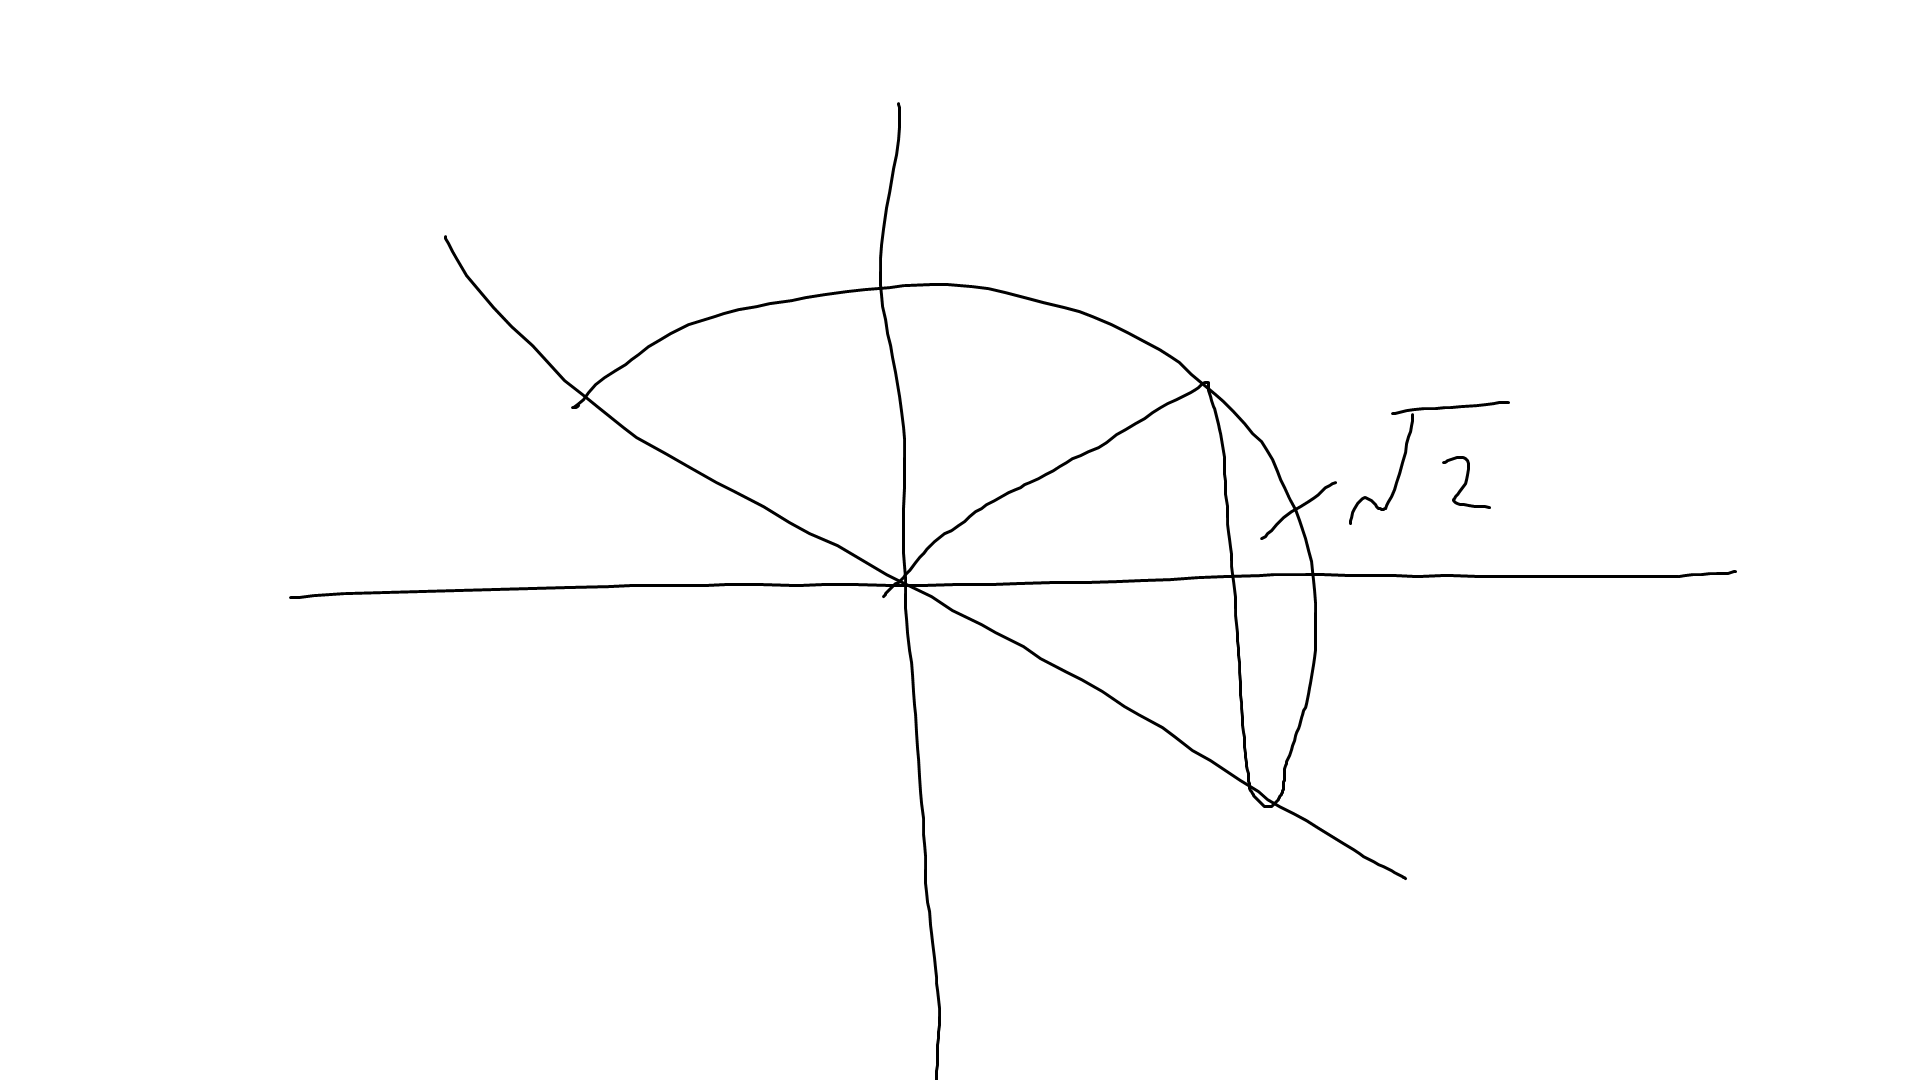
\includegraphics[scale=0.4]{CA_10}

Since $\theta_{n-1} (a_{n-1}) = \theta_n (a_{n-1}) + 2\pi B_n$, where $B_n \in \Z$. So by adding suitable multiple of $2\pi$ to each $\theta_n$, we can make them match and fit together to get a continuous $\theta$.
\end{proof}
\end{thm}

Given such a continuous $\theta$, define 
\begin{equation*}
\begin{aligned}
I(\gamma,w) = \frac{\theta(b)-\theta(a)}{2\pi}
\end{aligned}
\end{equation*}
This is well-defined: if $\theta_1$, $\theta_2$ are two continuous functions s.t. (*) holds, then $\theta_1-\theta_2 \in 2\pi \Z$, so is constant by continuity.

If $\gamma$ is closed, i.e. $\gamma(b) = \gamma(a)$, then $I(\gamma,w) \in \Z$.

\begin{rem}
Other possible common notations are $n(\gamma,w)$ or $n_\gamma(w)$.
\end{rem}

If $\gamma$ is $C^1$ (or piecewise $C^1$), we can give directly a function $\theta$ which is also $C^1$ (or piecewise). Assume WLOG $w=0$. Then define
\begin{equation*}
\begin{aligned}
h(t) := \int_0^t \frac{\gamma'(s)}{\gamma(s)} ds
\end{aligned}
\end{equation*}
with
\begin{equation*}
\begin{aligned}
h'(t) = \frac{\gamma'(t)}{\gamma(t)}
\end{aligned}
\end{equation*}
So
\begin{equation*}
\begin{aligned}
\frac{d}{dt} \left(\gamma(t) e^{-h(t)} \right) = \gamma'(t) e^{-h} \gamma e^{-h} (-h') = e^{-h} (\gamma - h'\gamma) = 0
\end{aligned}
\end{equation*}
So $\gamma(t) e^{-h}$ is a constant. Write $\gamma(t) = \gamma(a) e^{h(t)}$. So $\theta(t) = \arg(\gamma(a)) + \Im h(t)$.

\begin{lemma} 3.2\\
Let $\gamma:[a,b] \to \C \setminus \{w\}$ closed and piecewise $C^1$ curve. Then
\begin{equation*}
\begin{aligned}
I(\gamma,w) = \frac{1}{2\pi i}\int_\gamma \frac{dz}{z-w}.
\end{aligned}
\end{equation*}
\begin{proof}
$\gamma(t) = w+\gamma(t) e^{i\theta(t)}$ with $r$ and $\theta$ pieciwise $C^1$. Then
\begin{equation*}
\begin{aligned}
\int_\gamma \frac{dz}{z-w} &= \int_a^b \frac{\gamma'(t)}{\gamma(t)-w} dt \\
&= \int_a^b \left(\frac{r'}{r} + i\theta'\right) dt\\
&= \left[\log r(t) + i\theta(t)\right]_a^b\\
&= i(\theta(b)-\theta(a))\\
&= 2\pi i I(\gamma,w).
\end{aligned}
\end{equation*}
\end{proof}
\end{lemma}

\begin{coro} 3.3\\
(1) $I(\gamma,w)$ is constant on each path-component on $\C\setminus \gamma([a,b])$.\\
(2) If $w$ is in the unique unbounded component of $\C\setminus \gamma([a,b])$ then $I(\gamma,w)=0$.
\begin{proof}
(1) Note $\C \setminus \gamma([a,b]) \to I(\gamma,w)$ is continuous.\\ (Check that 
\begin{equation*}
\begin{aligned}
\frac{1}{2\pi i} \int_\gamma \frac{dz}{z-w}
\end{aligned}
\end{equation*}
we can argue just as we did a couple of lectures ago when proving the CIF for $f'(w)$).\\
Since it takes value in $\Z$, it must be constant on each component.

(2) $\gamma([a,b])$ is compact, so there exists a unique unbounded component. Then
\begin{equation*}
\begin{aligned}
|I(\gamma,w)| = \frac{1}{2\pi} \left|\int_\gamma \frac{dz}{z-w}\right| \leq \frac{length(\gamma)}{2\pi} \sup_{z \in r} \frac{1}{|z-w|} \leq \frac{length(\gamma)}{2\pi \frac{|w|}{2}}
\end{aligned}
\end{equation*}
as $|w| \to \infty$. The last inequality holds since $w \in \{z \in \C: |z|>2\max|u|, u \in \gamma([a,b]) \}$.
\end{proof}
\end{coro}

\subsection{General form of Cauchy's theorem (homotopy version)}
\begin{defi}
Let $\phi:[a,b] \to U$, $\psi:[a,b] \to U$ be piecewise \emph{closed} paths. A \emph{homotopy} from $\phi$ to $\psi$ is a map $F:[0,1] \times [a,b] \to U$ s.t\\
(i) $F$ is continuous;\\
(ii) $F|_{\{0\} \times [a,b]} = \phi, F_{\{1\} \times [a,b]} = \psi$;\\
(iii) $\forall s \in [0,1]$, $F_s(t) = F(s,t): [a,b] \to U$ is closed and piecewise $C^1$.

This is like some continuous transform of $\phi$ into $\psi$, where the first argument of $F$ is the 'time'; so the second condition marks the starting shape and end ending shape.
\end{defi}

\begin{defi}
A domain $U$ is simply connected if every piecewise $C^1$ closed path $\gamma:[a,b] \to U$ is homotopic to a constant path (i.e. a point).

We can think of this as: any curve can be continuously shrinked into one point.
\end{defi}

\begin{rem}
A star-domain is simply connected.
\end{rem}

\begin{rem} (*)
$U$ simply connected is also equivalent with:\\
(1) $I(\gamma,w) = 0$ for all closed curves $\gamma$ in $U$ and $w \not\in U$;\\
(2) $U \subset \C_\infty$, the complemment of $U$ is connected in $\C_\infty$;
\end{rem}

\begin{defi}
Let $\phi:[0,1] \to U$ and $\psi: [0,1] \to U$ be paths. Then $\psi$ is an \emph{elementary deformation} of $\phi$ if\\
(i) $\exists x_0 = 0<x_1 < ... < x_n = 1$ and \emph{convex open sets} $C_1,...,C_n \subset U$ s.t. for $t \in [x_{i-1},x_i]$, $\phi(t)$ and $\psi(t) \in C_i$.

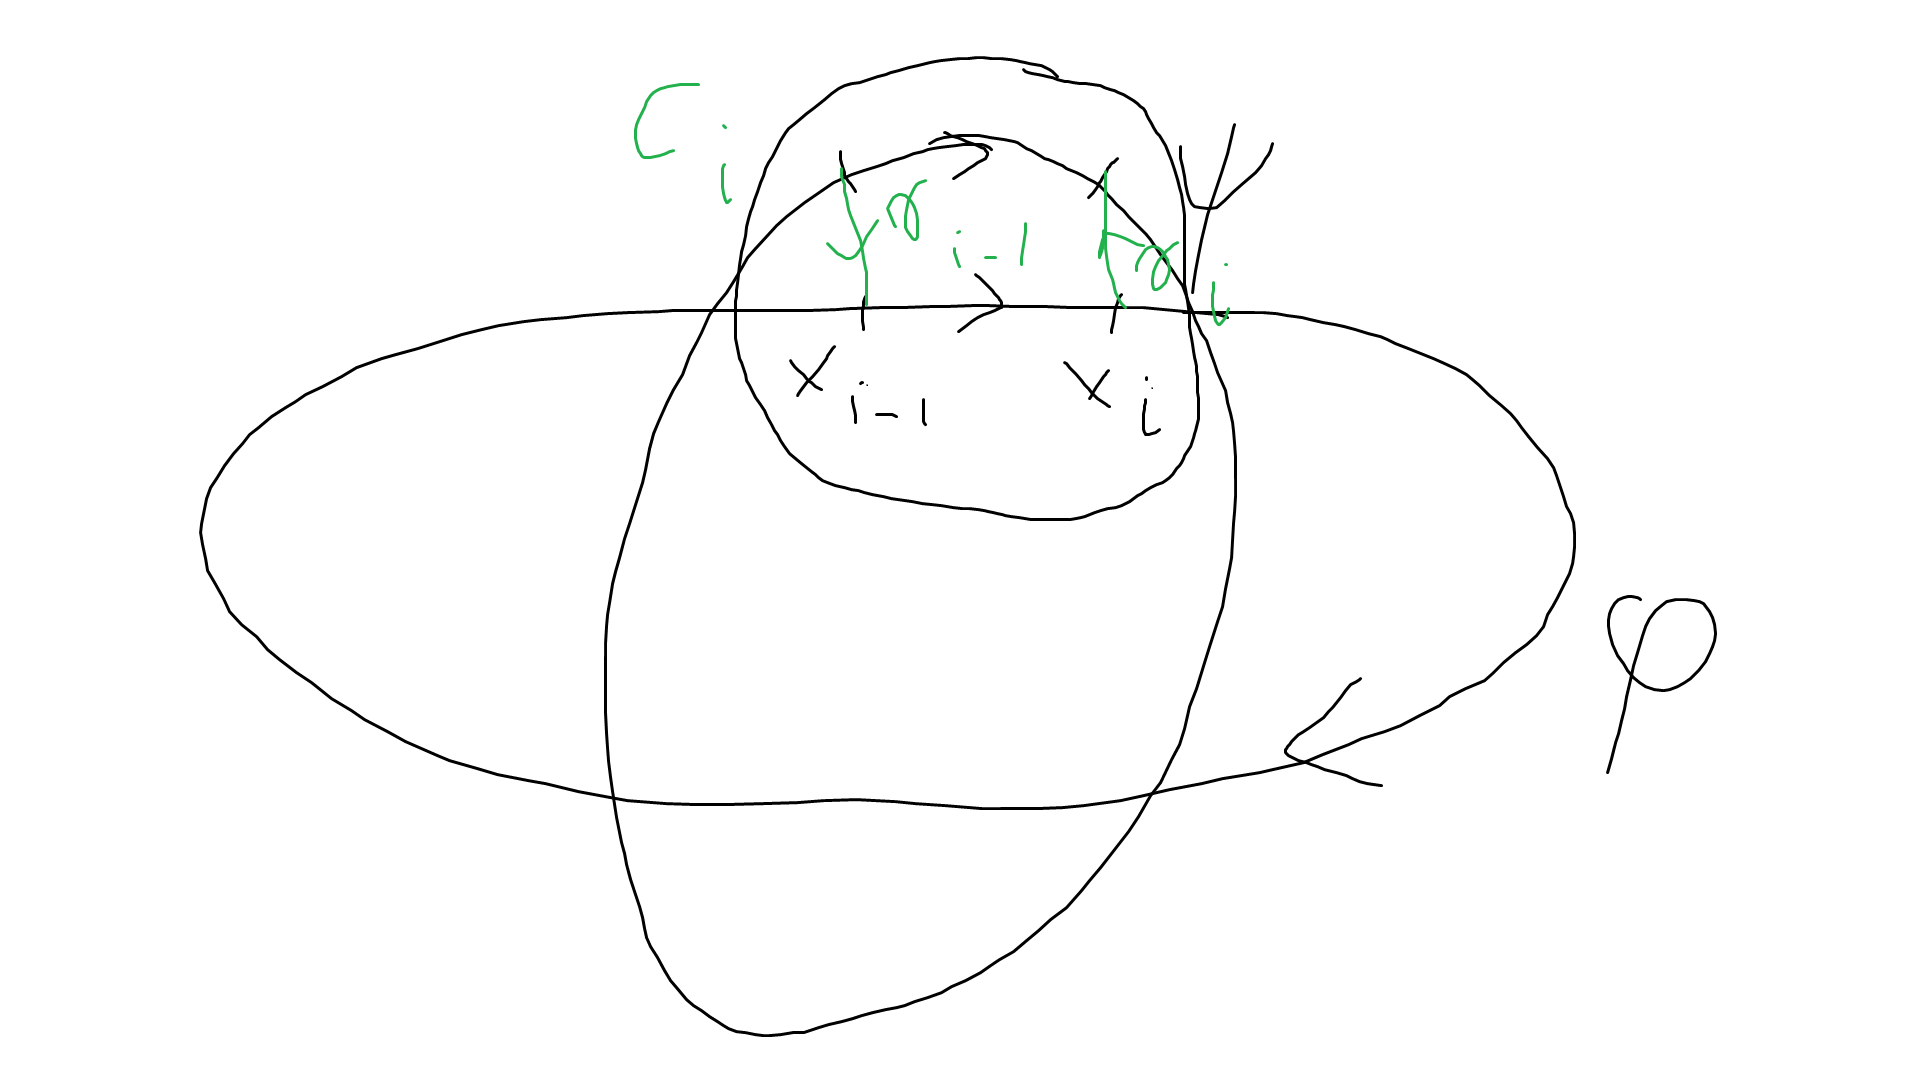
\includegraphics[scale=0.4]{CA_11}
\end{defi}

Let $\phi_i = \phi|_{[x_{i-1},x_i]}$, $\psi_i = \psi|_{[x_{i-1},x_i]}$. Let $\gamma_i$ be a straight line segment from $\phi(x_i)$ to $\psi(x_i$).

Convex Cauchy:

\begin{equation*}
\begin{aligned}
\int_{\phi_i+\gamma_i - \psi_i - \gamma_{i-1}} f(z)dz = 0
\end{aligned}
\end{equation*}
for $f$ holomorphic.

If we sum over $i$ from $1$ to $n$, we obtain
\begin{equation*}
\begin{aligned}
\int_\phi f(z) dz = \int_\psi f(z) dz
\end{aligned}
\end{equation*}
(integrals over $\gamma_i$ cancel in pairs).

\begin{prop} 3.4\\
If $\phi$ and $\psi$ are homotopic closed paths in a domain $U$, then there are $\phi = \phi_1,...,\phi_N = \psi$ s.t. $\phi_{i+1}$ is an elementary deformation of $\phi_i$.
\end{prop}

This proposition and the previous argument give
\begin{thm} 3.5 (Homotopy form of Cauchy's theorem)\\
Let $f:U \to \C$ be holomorphic. If $\phi,\psi$ are homotopic closed paths, then
\begin{equation*}
\begin{aligned}
\int_\phi f(z) dz = \int_\psi f(z) dz.
\end{aligned}
\end{equation*}
In particular, if $\gamma$ is homotopic to a constant path, then $int_\gamma f(z) dz = 0$.
\end{thm}

\begin{coro} 3.6\\
let $U$ be a simply-connected domain and $f:U \to \C$ holomorphic. Then
\begin{equation*}
\begin{aligned}
\int_\gamma f(z) dz = 0
\end{aligned}
\end{equation*}
for all closed paths $\gamma$.
\end{coro}

\begin{proof} (of proposition 3.4) (exercise on uniform continuity)\\
Let $F: [0,1]\times [a,b] \to U$ be the homotopy between $\phi$ and $\psi$. We know $\im(F)$ is compact. The distance between $\im(F)$ and $\C\setminus U$ is $\varepsilon>0$. Hence $D(F(s,t),\varepsilon) \subset U$ $\forall (s,t)$.

$F$ is uniformly continuous, so given $\varepsilon>0$, $\exists \delta>0$ s.t. $|(s,t)-(s',t')|<\delta \implies |F(s,t)-F(s',t')| < \varepsilon$.

Pick $N$ s..t $\frac{1+(b-a)}{n} < \delta$ and set $x_j = a+\frac{(b-a)j}{n}$ for $j=1,...,n$. Let
\begin{equation*}
\begin{aligned}
\phi_i = F|_{\{1/n\} \times [a,b]}
\end{aligned}
\end{equation*}
Then
\begin{equation*}
\begin{aligned}
C_{ij} = D(F(1/n,x_j),\varepsilon)
\end{aligned}
\end{equation*}
are convex. If $s \in [\frac{i-1}{n},\frac{i}{n}]$,$t\in[x_{j-1},x_j]$, then $F(s,t) \in C_{ij}$ because of the uniform continuity equation. So $\phi_i$ is an elementary deformation of $\phi_{i-1}$.
\end{proof}

\newpage

\section{Singularities, Laurent expansions and the residue theorem}

\subsection{Laurent expansions}

\begin{thm} 4.1\\
Let $f$ be holomorphic on an annulus $A = \{z \in \C: r<|z-a|<R\}$ for $0\leq r < R \leq \infty$. Then\\
(i) $f$ has a unique convergent series expansion on $A$
\begin{equation*}
\begin{aligned}
f(z) = \sum_{n=-\infty}^\infty c_n(z-a)^n;
\end{aligned}
\end{equation*}
(ii) For any $\rho \in (r,R)$, the coefficient $c_n$ is given by
\begin{equation*}
\begin{aligned}
c_n = \frac{1}{2\pi i}\int_{|z-a|=\rho} \frac{f(z)}{(z-a)^{n+1}} dz;
\end{aligned}
\end{equation*}
(iii) If $r < \rho' \leq \rho < R$, then the series converges uniformly on the set $\{z \in \C: \rho'\leq |z-a|\leq \rho\}$ (hence locally uniformly in $A$).
\begin{proof}
As in the proof of the CIF, we consider the following function: if $w \in A$,
\begin{equation*}
\begin{aligned}
g(z) = \left\{\begin{array}{ll}
\frac{f(z)-f(w)}{z-w} & z \neq w\\
f'(w) & z = w
\end{array}\right.
\end{aligned}
\end{equation*}
$g$ is holomorphic in $A$ (follows from results in previous lectures). Choose $r<p\rho_2 < |w-a|<\rho_1<R$, $C_1:|z-a|=\rho_1$, $C_2:|z-a| = \rho_2$. By theorem 3.5 ($C_1$ and $C_2$ are homotopic in $A$),
\begin{equation*}
\begin{aligned}
&\int_{C_1} g(z) dz =\int_{C_2} g(z) dz\\
\implies &\int_{C_1} \frac{f(z)}{z-w} dz - f(w) \int_{C_1} \frac{dz}{z-w} (=2\pi i I(C_1,w)=1) \\
= &\int_{C_2}\frac{f(z)dz}{z-w} - f(w) \int_{C_2}\frac{dz}{z-w}(=2\pi i I(C_2,w)=0)
\end{aligned}
\end{equation*}
So
\begin{equation*}
\begin{aligned}
f(w) = \frac{1}{2\pi i}\int_{C_1} \frac{f(z)}{z-w}dz - \frac{1}{2\pi i}\int_{C_2} \frac{f(z) dz}{z-w}
\end{aligned}
\end{equation*}

Let the first integral be $f_1(w)$ and the second be $f_2(w)$. For $f_1$, expand just as in the proof of Taylor series to get
\begin{equation*}
\begin{aligned}
f_1(w) = \sum_{n=0}^\infty c_n (w-a)^n
\end{aligned}
\end{equation*}
where $$c_n = \frac{1}{2\pi i} \int_{C_1} \frac{f(z)}{(z-a)^{n+1}} dz$$ $\forall n \geq 0$ ($\frac{1}{z-w} = \sum_{n=0}^\infty \frac{(w-a)^n}{(z-a)^{n+1}}$).

For $f_2$ we use
\begin{equation*}
\begin{aligned}
\frac{-1}{z-w} = \frac{1/w-a}{1-\frac{z-a}{w-a}} = \sum_{m=1}^\infty \frac{(z-a)^{m-1}}{(w-a)^m}
\end{aligned}
\end{equation*}
which converges uniformly for $|z-a|=\rho_2$, giving
\begin{equation*}
\begin{aligned}
f_2(w) = \sum_{m=1}^\infty d_m (w-a)^{-m}
\end{aligned}
\end{equation*}
where
\begin{equation*}
\begin{aligned}
d_m = \frac{1}{2\pi i} \int_{C_2} \frac{f(z)}{(z-a)^{-m+1}} dz
\end{aligned}
\end{equation*}
$\forall m\geq 1$. Writing $n=-m$ we get part (i).
\end{proof}
\end{thm}

(missing two lectures)

Let $f:U \setminus \{z_1,...,z_k\} \to \C$ be holomorphic, $U$ simply connected, $z_i \not\in \im(\gamma)$, $\gamma$ closed. Then
\begin{equation*}
\begin{aligned}
\frac{1}{2\pi i} \int_\gamma f(z) dz = \sum_i I(\gamma,z_i) Res_{z_i} f
\end{aligned}
\end{equation*}
Some observations about computing residues:\\
(i) Simple pole at $a$: $Res_a f = \lim_{z \to a} (z-a) f(z)$;\\
(ii) $f = g/h$, $g,h$ are holomorphic, $g(a) \neq 0$, $a$ simple zero of $h$, then $$Res_a f = \frac{g(a)}{h'(a)};$$
(iii) $f(z) = (z-a)^{-k} g(z)$, with $g$ holomorphic, then $Res_a f = \frac{g^{(k-1)}(a)}{(k-1)!} = $ coefficient of $(z-a)^{k-1}$ in Taylor expansion for $g$.

\begin{eg}
Consider
\begin{equation*}
\begin{aligned}
\int_{-\infty}^\infty \frac{\cos x}{1+x+x^2} dx.
\end{aligned}
\end{equation*}

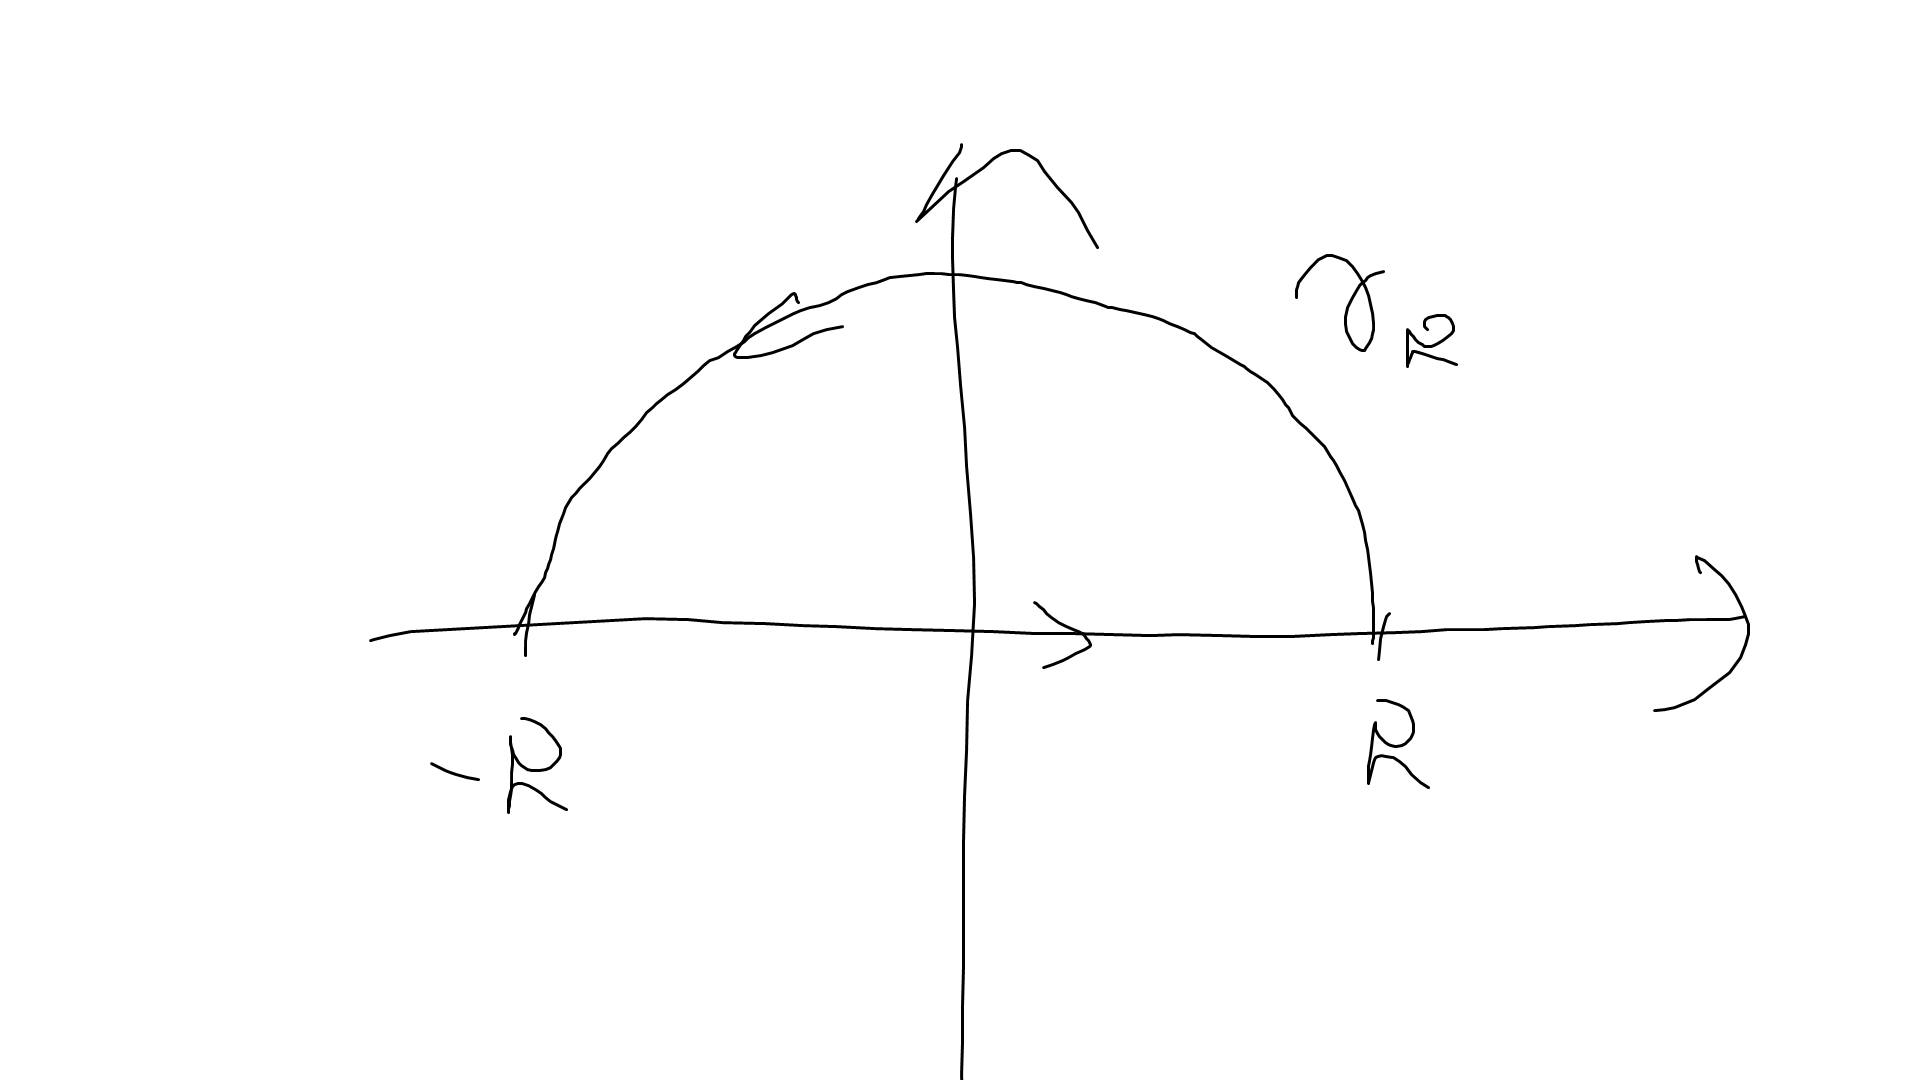
\includegraphics[scale=0.4]{CA_13}

Let $f(z) = \frac{e^{iz}}{1+z+z^2}$. $f$ has a simple pole at $w = e^{2\pi i/3}$. We have
\begin{equation*}
\begin{aligned}
Res_w f = \frac{e^{iw}}{2w+1}
\end{aligned}
\end{equation*}
On the semicircle $Re^{i\theta}$ for $\theta \in [0,\pi]$,
\begin{equation*}
\begin{aligned}
\left|\int_0^\pi f(Re^{i\theta}) Rie^{i\theta} d\theta\right| &\leq \int_0^\pi |f(Re^{i\theta})| R d\theta\\
&= R\int_0^\pi \frac{e^{-R\sin\theta}}{|R^2 e^{2i\theta}+Re^{i\theta}+1|}d\theta\\
&= O(1/R) \to 0
\end{aligned}
\end{equation*}
as $R \to \infty$.

By using the residue theorem, 
\begin{equation*}
\begin{aligned}
\int_{-\infty}^\infty \frac{\cos x}{1+x+x^2} dx &= \Re\left(\int_\R f(z) dz\right)\\
&= \Re\left(\frac{2\pi i+e^{iw}}{2w+1}\right)\\
&= \frac{2\pi}{\sqrt{3}} \cos(1/2) e^{-\sqrt{3}/2}
\end{aligned}
\end{equation*}
\end{eg}

Two useful lemmas for estimating the integrals:

\begin{lemma} 4.8\\
Let $f$ be holomorphic on $D(a,R) \setminus \{a\}$, with a simple pole at $a$. If $0<\varepsilon<R$, let $\gamma:[\alpha,\beta] \to \C$ be $\gamma_\varepsilon(t) = a+\varepsilon e^{it}$. Then
\begin{equation*}
\begin{aligned}
\lim_{\varepsilon \to 0} \int_{\gamma_\varepsilon} f(z) dz = (\beta-\alpha) i Res_a f.
\end{aligned}
\end{equation*}

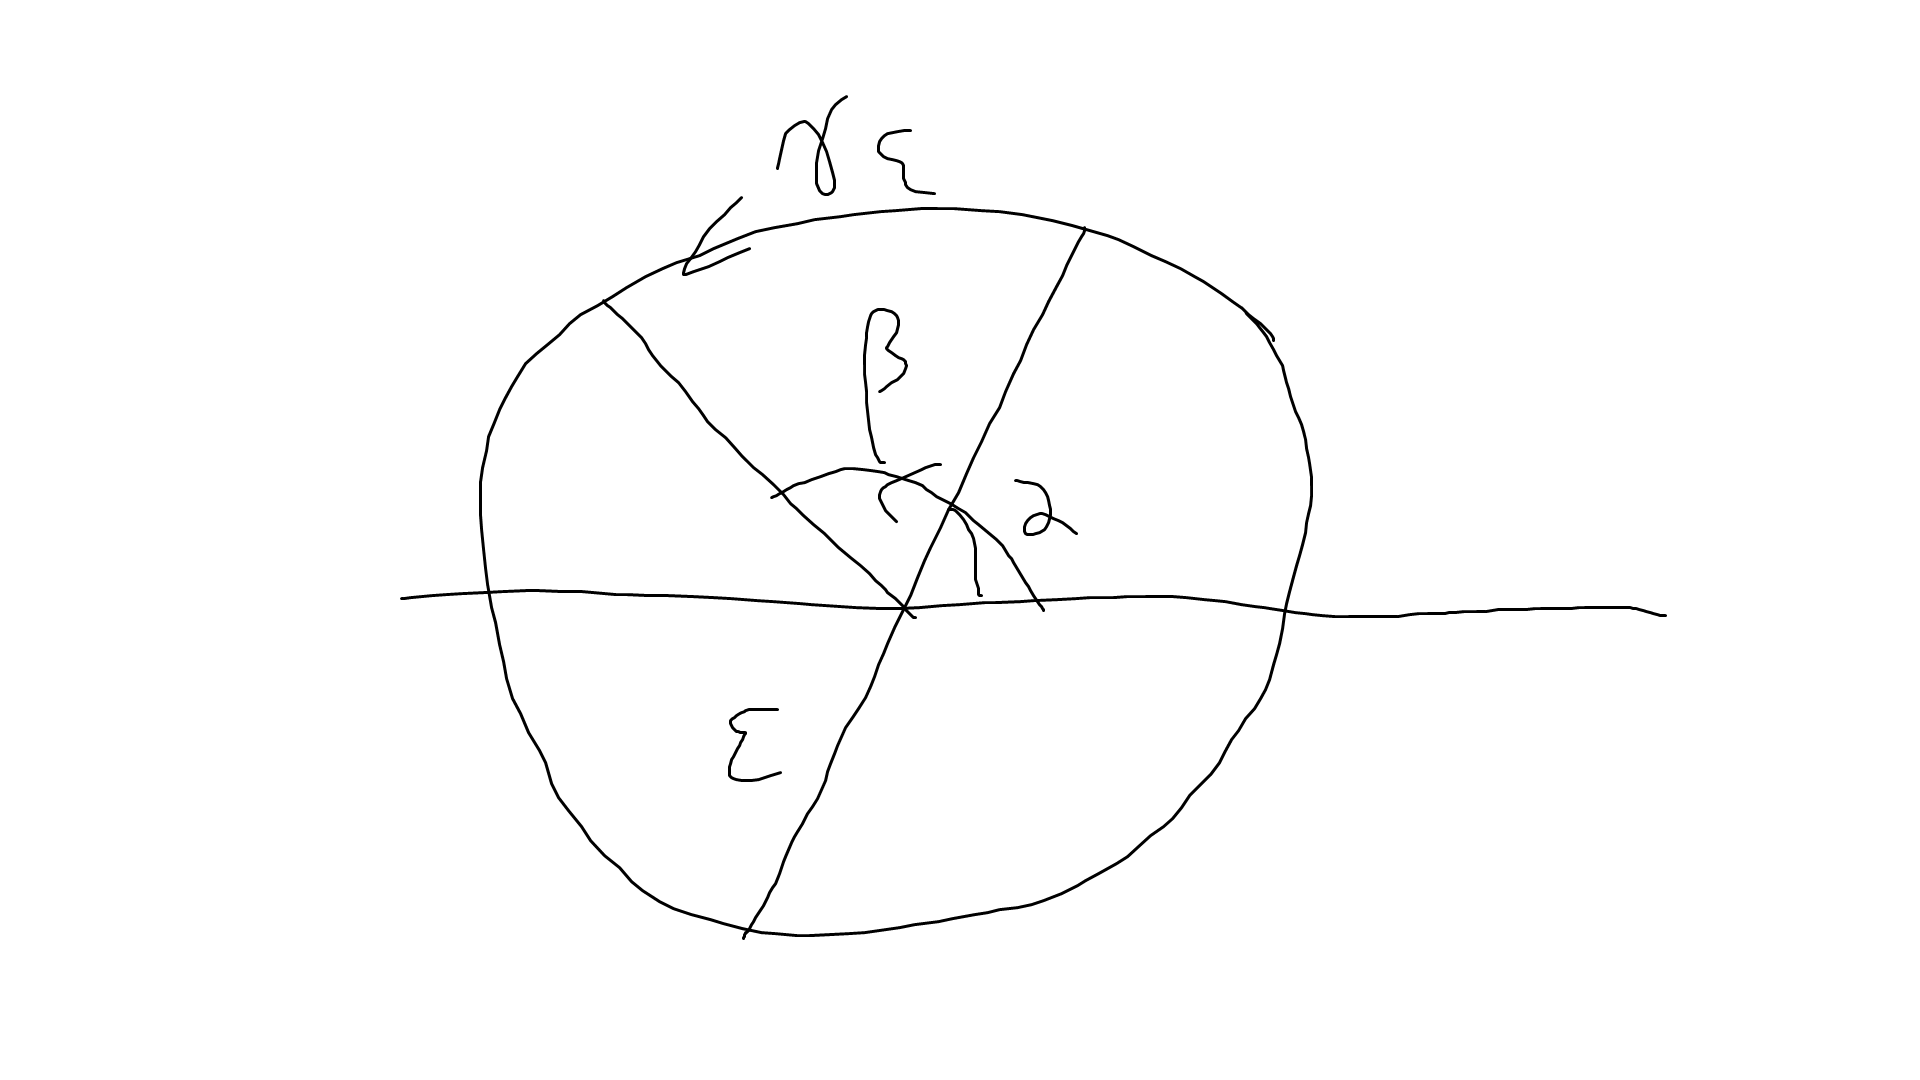
\includegraphics[scale=0.4]{CA_14}

\begin{proof}
Let $f(z) = \frac{c}{z-a} + g(z)$ with $g$ holomorphic in $D(a,R)$, and $c=Res_a f$. Then
\begin{equation*}
\begin{aligned}
\left|\int_{\gamma_\varepsilon} g(z) dz\right| &\leq (\beta-\alpha)\varepsilon \sup_{\gamma_z} |g(z)| \to 0
\end{aligned}
\end{equation*}
as $\varepsilon \to 0$ (since $g$ is continuous on $D(a,R)$, the supremum is bounded). But
\begin{equation*}
\begin{aligned}
\lim_{\varepsilon \to 0} \int_{\gamma_\varepsilon} \frac{c}{z-a} dz &=c \lim_{\varepsilon \to 0} \int_\alpha^\beta \frac{i\varepsilon e^{it}}{\varepsilon e^{it}} dt = (\beta-\alpha)i.
\end{aligned}
\end{equation*}
\end{proof}
\end{lemma}

\begin{lemma} 4.9 (Jordan's lemma)\\
If $f$ is holomorphic on $\{|z|>r\}$, and $z f(z)$ is bounded for large $|z|$, then $\forall \alpha > 0$,
\begin{equation*}
\begin{aligned}
\int_{\gamma_R} f(z) e^{i\alpha z} dz \to 0
\end{aligned}
\end{equation*}
as $R\to \infty$, where $\gamma_R(t) = Re^{it}$ for $t \in [0,\pi]$.
\begin{proof}
$|f(z)| \leq \frac{c}{|z|}$ for large $|z|$, where $c$ is the same constant. On $(0,\frac{\pi}{2}]$,
\begin{equation*}
\begin{aligned}
\frac{d}{d\theta}\left(\frac{\sin\theta}{\theta}\right) = \frac{\theta \cos \theta - \sin\theta}{\theta} \leq 0
\end{aligned}
\end{equation*}
So $\frac{\sin\theta}{\theta}$ decreases and hence $\sin t \geq \frac{2t}{\pi}$ for $t \in [0,\frac{\pi}{2}]$. Then
\begin{equation*}
\begin{aligned}
|e^{i\alpha z}| = e^{-R\alpha \sin t} \leq \left\{\begin{array}{ll}
e^{-\frac{R\alpha 2t}{\pi}} & 0 \leq t \leq \frac{\pi}{2}\\
e^{-\frac{R\alpha 2t'}{\pi}} & 0 \leq t' = \pi-t \leq \frac{\pi}{2}
\end{array}\right.
\end{aligned}
\end{equation*}
For the $1/4-$circle in the first quadrant, let $z=e^{it}$. Then
\begin{equation*}
\begin{aligned}
\left|\int_0^{\pi/2} e^{i\alpha Re^{it}} f(Re^{it}) iRe^{it} dt\right| &\leq \int_0^{\pi/2} ce^{-\frac{2Rt\alpha}{\pi}} dt\\
&= \frac{c\pi}{2R\alpha} [1-e^{-R\alpha} \to 0
\end{aligned}
\end{equation*}
as $R \to \infty$. Same for the other $1/4-$circle.
\end{proof}
\end{lemma}

\begin{eg} (see CM sheet)\\
$\int_0^\infty \frac{\sin x}{x} dx$.

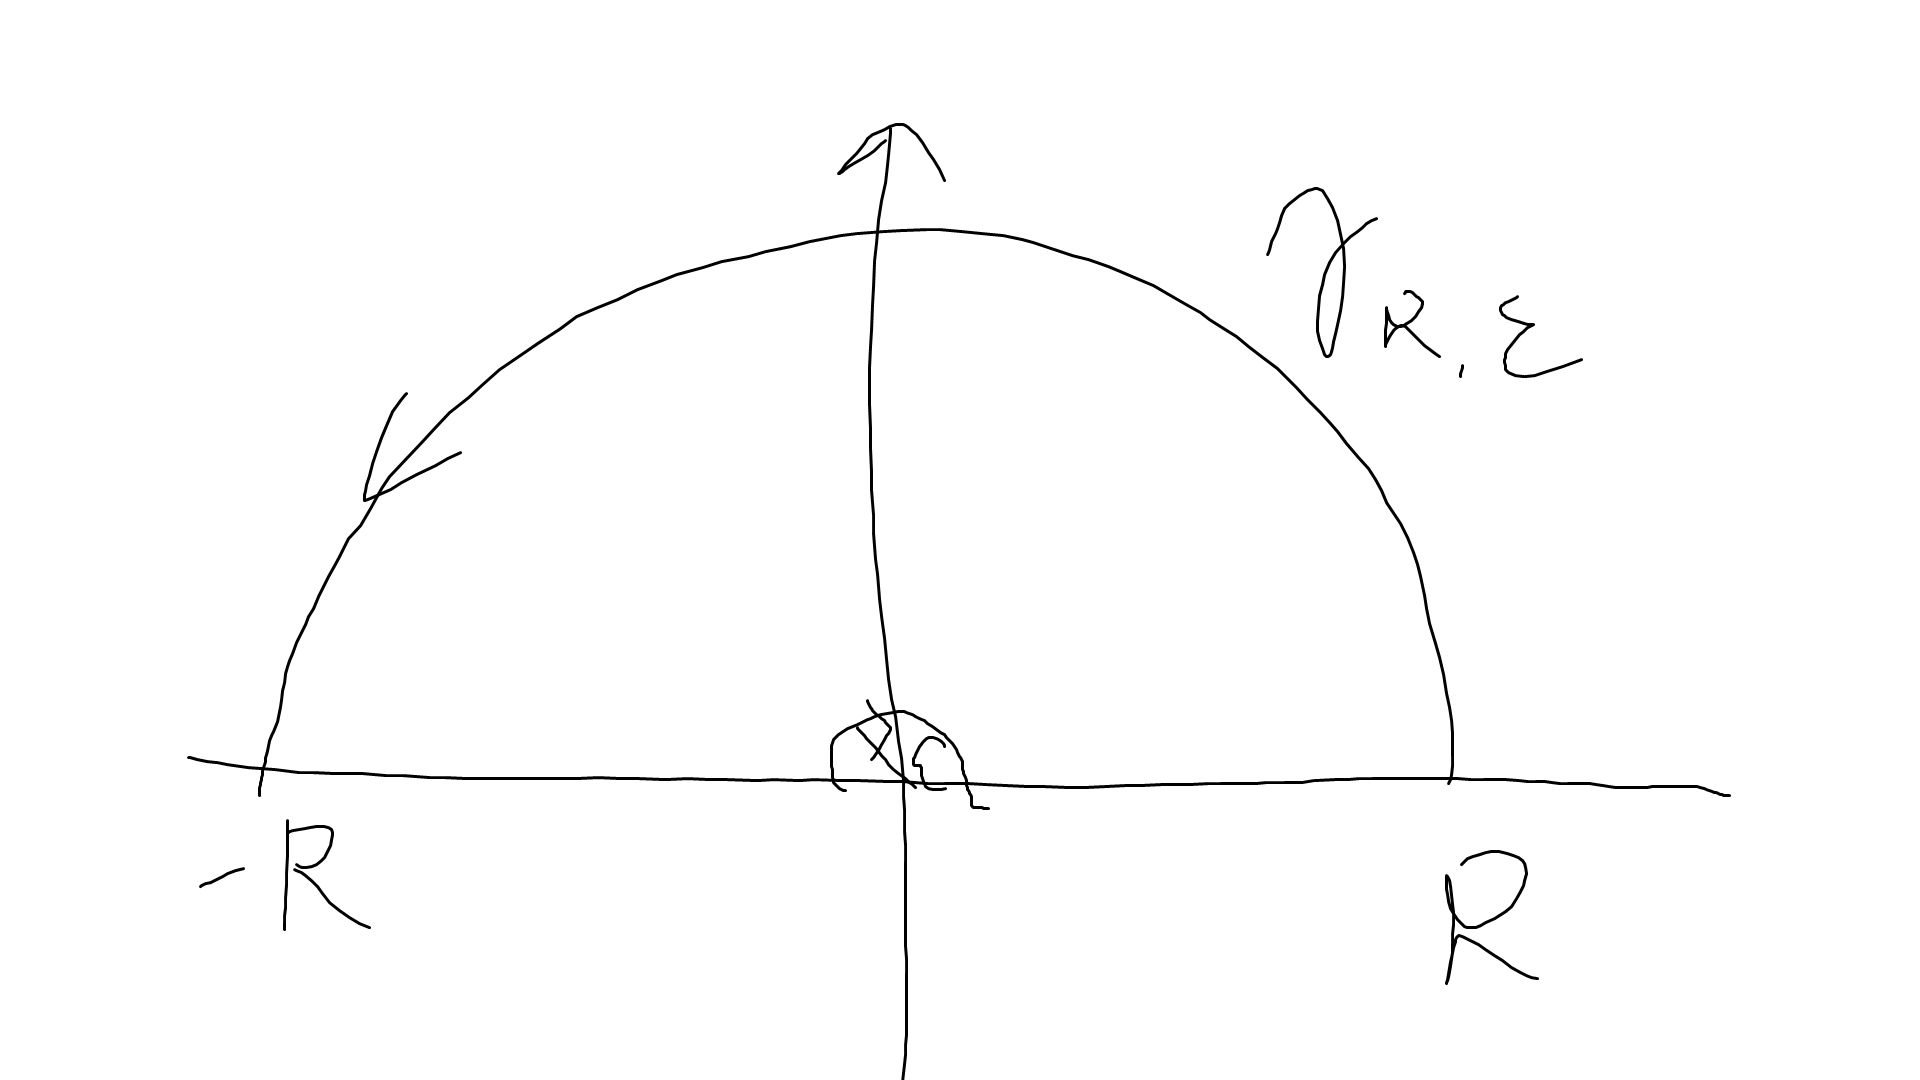
\includegraphics[scale=0.4]{CA_15}

Let $f(z) = \frac{e^{iz}}{z}$. Then
\begin{equation*}
\begin{aligned}
\int_{\gamma_{R,\varepsilon}} f(z) dz = 0,\\
\int \frac{e^{iz}}{z} dz \to 0
\end{aligned}
\end{equation*}
as $R \to \infty$ by Jordan's lemma.
\begin{equation*}
\begin{aligned}
\lim_{\varepsilon \to 0} \int f(z) dz = -\pi i
\end{aligned}
\end{equation*}
$Res_0 f=1$, $\frac{\sin x}{x}$ is even. So
\begin{equation*}
\begin{aligned}
\int_0^\infty \frac{\sin x}{x} = \frac{\pi}{2}.
\end{aligned}
\end{equation*}
\end{eg}

\begin{eg}
\begin{equation*}
\begin{aligned}
I = \int_0^{\frac{\pi}{2}} \frac{dt}{1+\sin^2 t}.
\end{aligned}
\end{equation*}
We have
\begin{equation*}
\begin{aligned}
\sin t = \frac{e^{it}-e^{-it}}{2i}
\end{aligned}
\end{equation*}
hence if $|z|=1$, $|z| = e^{it}$, $\sin t = \frac{z-1/z}{2i}$, $\frac{dz}{dt} = ie^{it}$. Then
\begin{equation*}
\begin{aligned}
\int_0^{\pi/2} \frac{dt}{1+\sin^2 t} &= \frac{1}{4} \int_0^{2\pi} \frac{dt}{1+\sin^2t}\\
&= \frac{1}{4} \int_{|z|=1} \frac{dz}{iz+\left[1+\frac{(z-1/z)^2}{-4}\right]}\\
&= \int_{|z|=1} \frac{iz dz}{z^4 - 6z^2 + 1} 
\end{aligned}
\end{equation*}

$y^2-6y+1$ has roots $3 \pm \sqrt{2}$, so $z^4 + 6z^2+1$ has roots $1\pm \sqrt{2},-1 \pm \sqrt{2}$. We see $1-\sqrt{2}$ and $-1+\sqrt{2}$ are inside the circle.

\begin{equation*}
\begin{aligned}
Res_{q_\pm} f = \frac{i q_\pm}{4q^3_\pm - 12q_\pm} = \frac{-i\sqrt{2}}{16}
\end{aligned}
\end{equation*}
So we get $I=\frac{\pi \sqrt{2}}{4}$.
\end{eg}

\newpage

\section{The Argument Principle, Rouch$\acute{e}$'s theorem}

\begin{prop} 5.1\\
Let $f$ have a zero (pole) of order $k$ at $z=a$. Then $f'(z)/f(z)$ has a simple pole at $z=a$ with residue $k$ (respectively $-k$).
\begin{proof}
Assume $f$ has a zero of order $k$ at $a$. So $f(z) = (z-a)^k g(z)$, where $g$ is holomorphic and $g(a) \neq 0$.

If we compute
\begin{equation*}
\begin{aligned}
\frac{f'(z)}{f(z)} = \frac{k}{z-a} + \frac{g'(z)}{g(z)}
\end{aligned}
\end{equation*}
where $g'(z)/g(z)$ is a nice holomorphic function near $a$. So $Ref_a f = k$.

For a pole we have $f(z) = (z-a)^{-k} g(z)$ and we get residue $-k$.
\end{proof}
\end{prop}

\begin{thm} 5.2 (Argument Principle)\\
Let $U$ be simply connected and suppose $f$ is a mesomorphic function on $U$ with finitely many zeros $\{z_1,...,z_k\}$ and poles $\{w_1,...,w_l\}$. Let $\gamma$ be a closed curve in $U$ s.t. $z_i,w_j \not\in \im(\gamma)$ $\forall i,j$. Then
\begin{equation*}
\begin{aligned}
\frac{1}{2\pi i} \int_\gamma \frac{f'(z)}{f(z)} dz = \sum_{i=1}^k I(\gamma,z_i) ord_{z_i}(f) - \sum_{j=1}^l I(\gamma,w_j) ord_{w_j} f
\end{aligned}
\end{equation*}
where $ord_{z_i} f$ and $ord_{w_j} f$ denotes the order of the respective zero or pole.
\begin{proof}
The function $f'/f$ is holomorphic except at isolated singularities given by $\{z_1,...,z_k\}$ and $\{w_1,...,w_l\}$. Hence we can apply the residue theorem combined with proposition 5.1 to prove the result.
\end{proof}
\end{thm}

\begin{rem}
Consider the curve $\Gamma = f \circ \gamma$ misses $0$. 

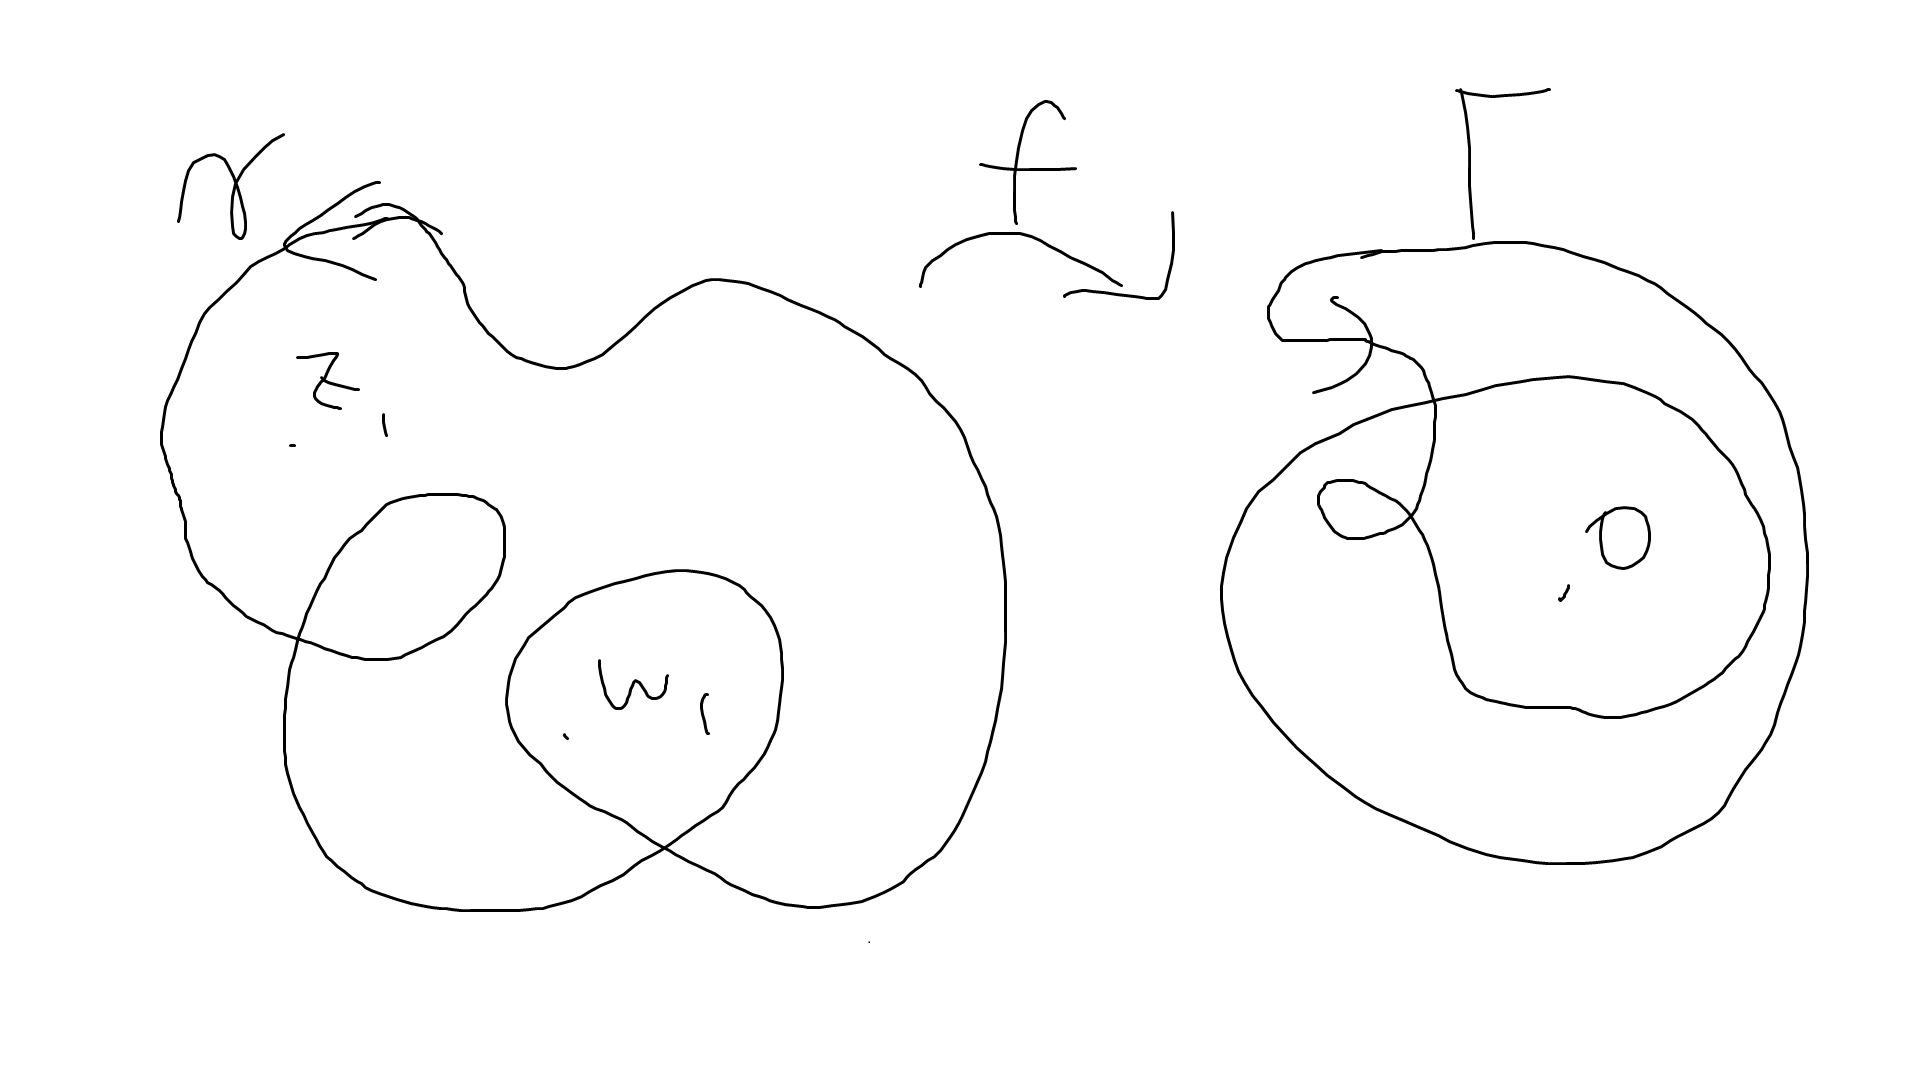
\includegraphics[scale=0.4]{CA_16}

Then
\begin{equation*}
\begin{aligned}
\frac{1}{2\pi i} \int_\gamma \frac{f'(z)}{f(z)} dz = \frac{1}{2\pi i} \int_\Gamma \frac{dw}{w} = I(\Gamma,0)
\end{aligned}
\end{equation*}
(Note $\frac{1}{2\pi i} \int_a^b \frac{f'(\gamma(t))\gamma'(t) dt}{f(\gamma(t))} = \frac{1}{2\pi i}\int_a^b \frac{\Gamma'(t)}{\Gamma(t)} dt$). So
\begin{equation*}
\begin{aligned}
I(\Gamma,0) = \sum_{i=1}^k I(\gamma,z_i) ord_{z_i} f - \sum_{j=1}^l I(\gamma,w_j) ord_{w_j} f
\end{aligned}
\end{equation*}

Now if we let $N$ be the number of zeros of $f$ inside $\gamma$ (counted with multiplicity), $P$ be the number of poles of $f$ inside $\gamma$ (same), then 
\begin{equation*}
\begin{aligned}
I(\Gamma,0) = N-P.
\end{aligned}
\end{equation*}

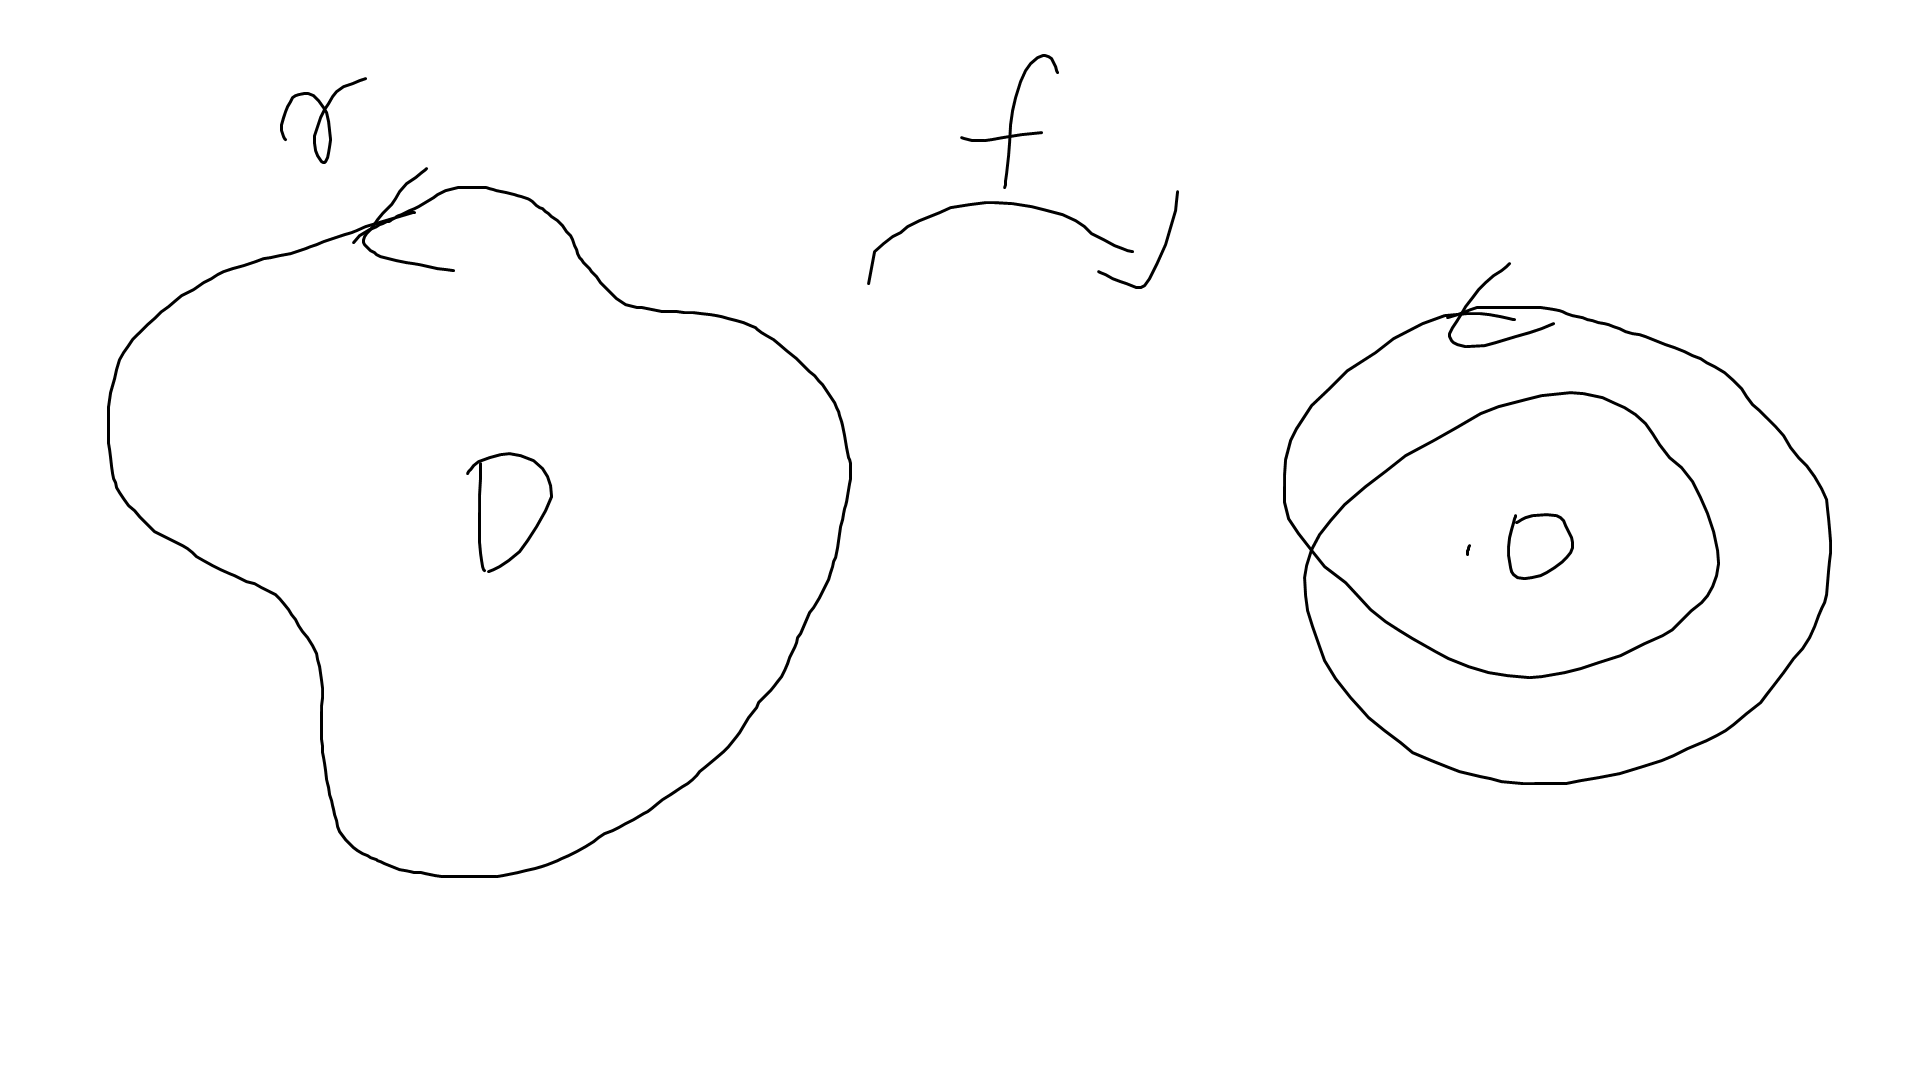
\includegraphics[scale=0.4]{CA_17}
\end{rem}

\begin{defi}
Let $\gamma$ be a closed curve in $U$. We say that $\gamma$ bounds a domain $D$ if $I(\gamma,w) = 1$ $\forall w \in D$ and $I(\gamma,w) = 0$ $\forall w \not\in D\cup\gamma$.
\end{defi}

Hence if $\gamma$ bounds a domain $D$, $I(\Gamma,0) = N-P$, where $N,P$ are the number of zeros and poles in $D$ respectively.

Consequences for the local behaviour of a holomorphic function:

Let $f$ be a \emph{non-constant} holomorphic function in some $U$. Take $a \in U$ and $f(a)=b$. We say that the local degree of $f$ at $a$ is the order of the zero of $f(z)-b$ at $z=a$ and denoted by $\deg_a (f)$, which is a positive integer.

\begin{prop} 5.3\\
The local degree of $f$ at $z=a$ equals $I(f_0 \gamma,f(a))$ for any circle $\gamma(t) = a+re^{2\pi it}$, $t \in [0,1]$ of sufficiently small radius (local model $z \to z^d$).
\begin{proof}
Apply Theorem 5.2 to $f(z)-f(a)$: This function has an isolated zero at $z=a$, hence it is non-zero in $0<|z-a|\leq r$ for $r$ sufficiently small.
\end{proof}
\end{prop}

\begin{thm} 5.4 (local mapping degree)\\
Let $f:D(a,R) \to \C$ be holomorphic and non-constant with local degree $\deg_a (f) = d>0$. Then if $r>0$ is sufficiently small, then there exists $\varepsilon>0$ s.t. for every $w$ with $0<|w-f(a)| \leq \varepsilon$, the equation $f(z) =w$ has exactly $d$ roots in $D(a,r)$.

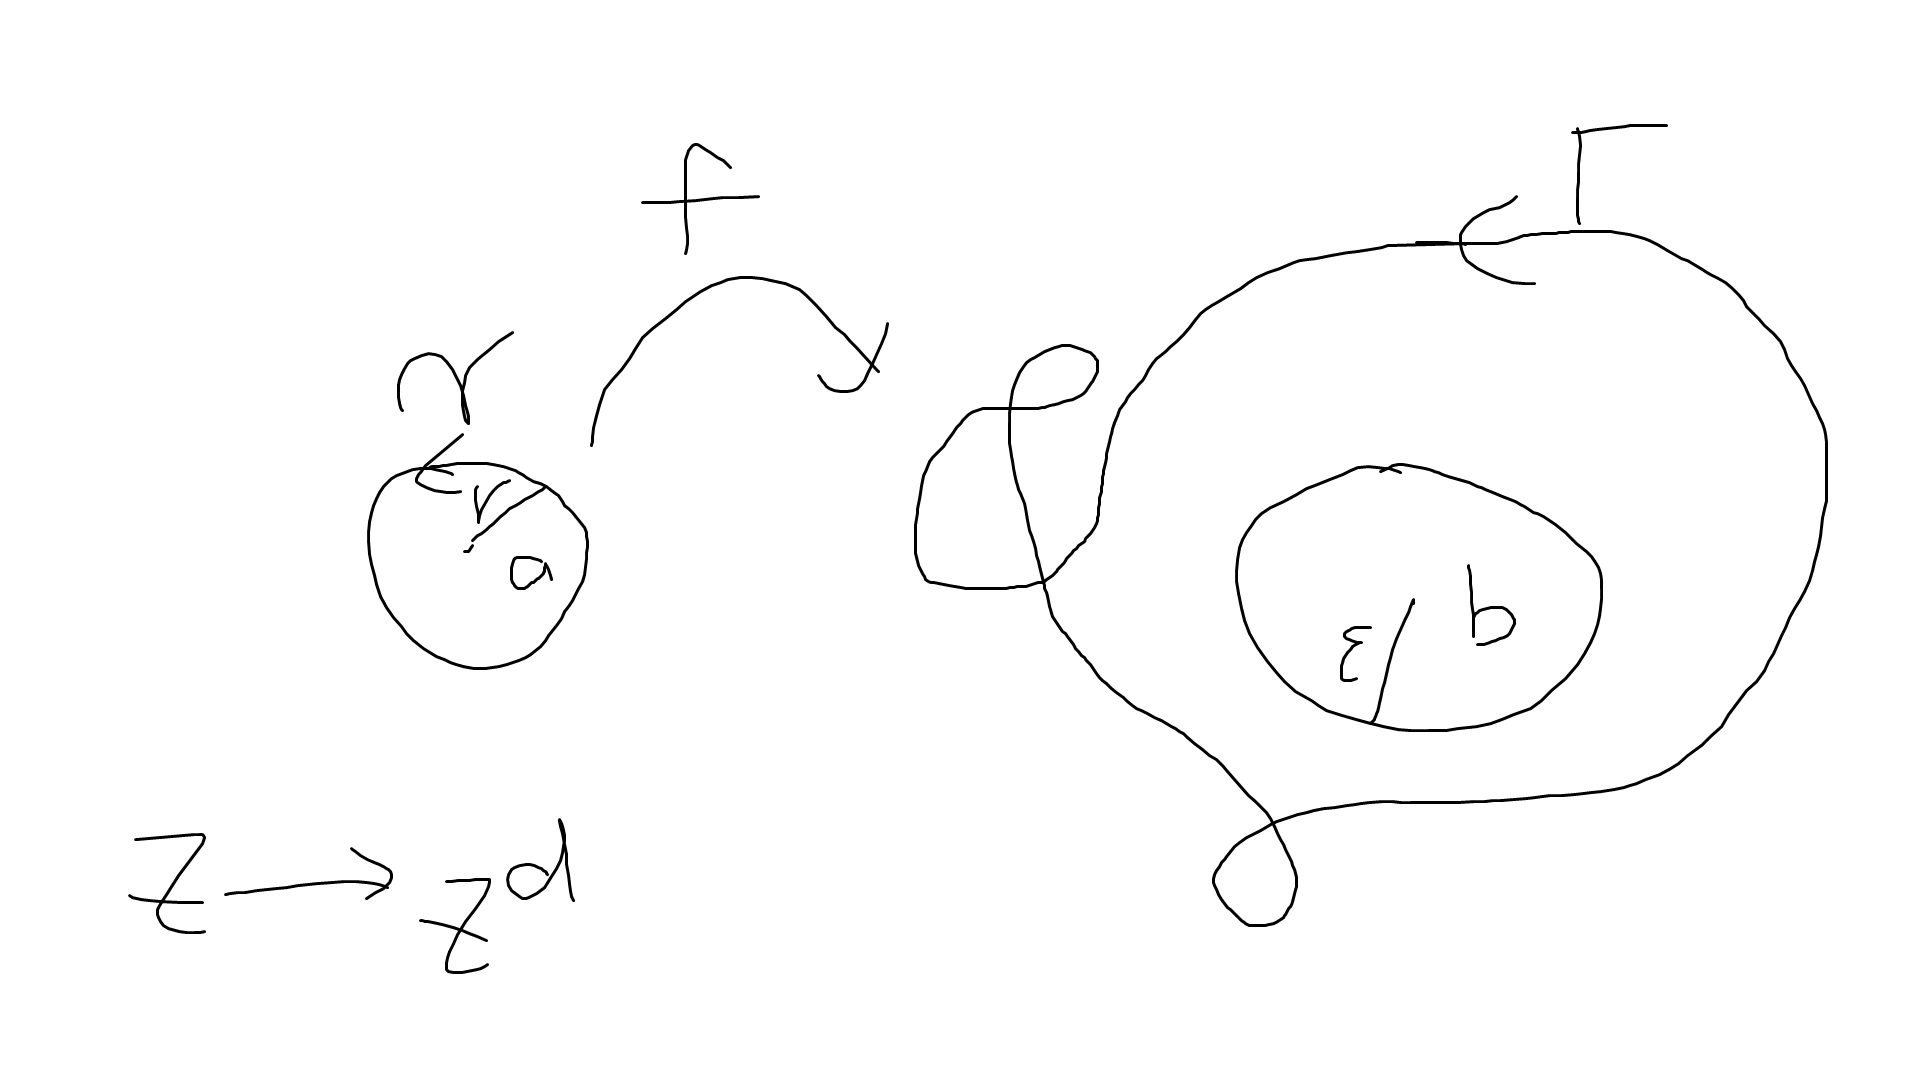
\includegraphics[scale=0.4]{CA_18}

(In the above diagram, every $w$ in the image has exactly $d$ preimages.)

\begin{proof}
Let $b=f(a)$. Let $r>0$ be s.t. both $f(z)-b$ and $f'(z)$ are non-zero for $0<|z-a|\leq r$.

Let $\gamma$ be the circle with center $a$ and radius $r$. Then $\Gamma=f\circ \gamma$ is a closed curve missing $b$. Choose $\varepsilon>0$ s.t. $D(b,\varepsilon)$ does not meet $\Gamma$ (image of $\Gamma$ is compact, hence its complement is open).

Then if $w \in D(b,\varepsilon)$, then the number of zeros (with multiplicity) of $f(z)-w$ in $D(a,r)$ equals $I(\Gamma,w)$ by the Argument principle. But $I(\Gamma,w) = I(\Gamma,b) = d$ by proposition 5.3.

Since $r$ was chosen so that $f'$ is non-zero on $D(a,r) \setminus \{a\}$, the zeros are all simple.
\end{proof}
\end{thm}

\begin{coro} 5.5 (open mapping theorem)\\
Let $f:U \to \C$ be holomorphic and non-constant. Then $f$ is an open mapping, that is, it maps open sets to open sets.
\begin{proof}
Let $V \subset U$ is open. We need to prove that $f(V)$ is open. Take $b \in f(V)$ and write it as $b=f(a)$, with $a \in V$.

But $V$ is open, so for $r$ sufficiently small, $D(a,r) \subset V$. The previous theorem gives $\varepsilon>0$ s.t.
\begin{equation*}
\begin{aligned}
D(b,\varepsilon) \subset f(D(a,r)) \subset f(V).
\end{aligned}
\end{equation*}
\end{proof}
\end{coro}

\begin{thm} 5.6 (Rouch$\acute{e}$'s theorem)\\
Let $f,g : U \to \C$ be holomorphic. Let $\gamma$ be a closed curve s.t. $\gamma$ bounds a domain $D$, and $|f| > |g|$ on $\gamma$. Then $f$ and $f+g$ have the same number of zeros in $D$.
\begin{proof}
Note that from the assumption, $f$ and $f+g$ do not have zeros on $\gamma$. Consider the function $h=1+g/f$.

R.T.P: $h$ has the same number of zeros ($N$) as poles($P$) in $D$.

By argument principle, $N-P = I(h\circ \gamma, 0)$. To finish the proof, need to show $I(h \circ \gamma,0) = 0$.

We have $|h-1|<1|$ on $\gamma$ by hypothesis, so $0$ lies in the unbounded component of the complement of the image of $h \circ \gamma$. So $I(h\circ \gamma,0) = 0$.
\end{proof}
\end{thm}

\begin{eg}
Consider polynomial $p(z) = z^4+6z+3$. At $|z|=2$, $|z^4|=16.15 = 6|z|+3 \geq |6z+3|$. Let $f=z^4$ and $g=6z+3$. Then by Rouch$\acute{e}$'s theorem, $z^4$ has the same number of zeros as $P$ inside $|z|<2$. So all roots of $P$ are inside $|z|<2$.

If we now look at $|z|=1$, then $6|z|+4 > 4 \geq |z^4+3|$. So $P(z)$ has the same number of roots as $6z$ inside $|z|<1$. So $P(z)$ has one root inside $|z|<1$ and 3 roots inside $1<|z|<2$.
\end{eg}

\newpage

\section{A Brief Summary of Our Theory}

From IA Analysis I we know about power series and radius of convergence. We proved some results about the criteria of complex differentiabilility (C-R equation) which also had something to do with harmonic functions and Laplace equations.

Then we proved some results about the existence of antiderivatives and being holomorphic: Cauchy's theorem for triangles; for star-domains; and for convex domains. Somewhere in between we proved the Fundamental Theorem of Calculus.

The next key idea was to go from the convex Cauchy to the Cauchy integral formula by considering the auxiliary function $g(z) = \frac{f(z)-f(w)}{z-w}$, and also yielding Liouville's theorem and Local maximum principle, as well as Taylor series which is helpful since holomorphic $\implies$ derivative is holomorphic. From there we get a connection to Converse Cauchy (Morera's theorem), and get that uniform limits of holomorphic functions are holomorphic.

The next stage of the course is topological in nature. We introduced two main topological ideas: index and homotopy. There we reach another highlight of the course (from local to global), the homotopy form of Cauchy's theorem. Then we discussed about Laurent Series and different types of singularities which yield the idea of residues and residue theorem that enabled us to do contour integrals. In the end we talked about the Argument pronciple, OMT, and Local degree theorem (with connection from Residue theorem).

\end{document}